%
% File eacl2021.tex
%
%% Based on the style files for ACL 2020, which were
%% Based on the style files for ACL 2018, NAACL 2018/19, which were
%% Based on the style files for ACL-2015, with some improvements
%%  taken from the NAACL-2016 style
%% Based on the style files for ACL-2014, which were, in turn,
%% based on ACL-2013, ACL-2012, ACL-2011, ACL-2010, ACL-IJCNLP-2009,
%% EACL-2009, IJCNLP-2008...
%% Based on the style files for EACL 2006 by 
%%e.agirre@ehu.es or Sergi.Balari@uab.es
%% and that of ACL 08 by Joakim Nivre and Noah Smith

\documentclass[11pt,a4paper]{article}
\usepackage[hyperref]{eacl2021}
\usepackage{times}
\usepackage{latexsym}
\renewcommand{\UrlFont}{\ttfamily\small}

% additional packages
\usepackage{float} % for floating
\usepackage{graphicx}% so it makes black blobs
\graphicspath{ {images/} }
\usepackage{caption}
\usepackage{subcaption}
\usepackage{amsmath}

\newenvironment{narrow}[2]{%
  \begin{list}{}{%
    \setlength{\topsep}{0pt}%
    \setlength{\leftmargin}{#1}%
    \setlength{\rightmargin}{#2}%
    \setlength{\listparindent}{\parindent}%
    \setlength{\itemindent}{\parindent}%
    \setlength{\parsep}{\parskip}%
  }%
  \item[]
}{\end{list}}


% This is not strictly necessary, and may be commented out,
% but it will improve the layout of the manuscript,
% and will typically save some space.
\usepackage{microtype}

\aclfinalcopy % Uncomment this line for the final submission
%\def\aclpaperid{***} %  Enter the acl Paper ID here

%\setlength\titlebox{5cm}
% You can expand the titlebox if you need extra space
% to show all the authors. Please do not make the titlebox
% smaller than 5cm (the original size); we will check this
% in the camera-ready version and ask you to change it back.

\newcommand\BibTeX{B\textsc{ib}\TeX}

\title{Bankruptcy Prediction: A Comparative Study on various Missing Value Imputation and Sampling Techniques}
% \title{Comparative Study on Different Missing Value Imputation and Resampling Techniques for Bankruptcy Prediction}

\author{
  Chirag Bhatt \\
  Department of Mathematics \\
  Indian Institute of Technology, Delhi \\
  Delhi 110016, India \\
  \texttt{mt1180750@maths.iitd.ac.in} \\\And
  Subhalingam D \\
  Department of Mathematics \\
  Indian Institute of Technology, Delhi \\
  Delhi 110016, India \\
  \texttt{mt1180770@maths.iitd.ac.in} \\}

\date{}

\begin{document}
\newcommand{\varrandomstate}{$2021$ }
% some placeholders
\newcommand{\varsplit}{$0.25$}
\newcommand{\varcrossval}{$2$}
\newcommand{\varcrossvalmetric}{F1-score }
\newcommand{\vasamplingstrategy}{$0.6$}
\newcommand{\vargithubrepo}{\url{https://github.com/cb3101/bankruptcy_prediction}}


%%% not used
\newcommand{\varacctrain}{$85.42\%$}
\newcommand{\varacctest}{$81.30\%$}
\newcommand{\varftrain}{$78.44\%$}
\newcommand{\varftest}{$74.72\%$}
\newcommand{\varprectrain}{$81.04\%$}
\newcommand{\varprectest}{$70.83\%$}
\newcommand{\varrectrain}{$76.00\%$}
\newcommand{\varrectest}{$79.06\%$}
\newcommand{\varlosstrain}{$0.33549$}
\newcommand{\varlosstest}{$0.43418$}


\maketitle
\begin{abstract}
This project aims towards experimenting with different methods for improving the existing models in the literature used for predicting corporate bankruptcy for Polish companies. More specifically, we aim to get better recall values as the existing models are suffering from poor recall. To tackle class imbalance, we use sampling techniques like SMOTE, RUS, SMOTE-ENN, and to impute missing values, we use Simple Imputer, MissForest, KNN. The performance of the models improved with SMOTE and simple imputation.\\

Keywords—Bankruptcy, Classification, SMOTE, 
Feature Selection, Imputation, Sampling
\end{abstract}


\section{Introduction}
\label{sec::intro}
Bankruptcy is a legal proceeding carried out to allow businesses unable to make payment to its creditors get freedom from their debts, while providing creditors an opportunity for repayment based on the business's assets. Only in USA more than 21 thousand businesses filed for bankruptcy in year 2020 [\href{https://www.investopedia.com/terms/b/bankruptcy.asp}{Investopedia}].  When a company becomes bankrupt and goes for into liquidation, stock shares becomes practically worthless. The common shareholders may, at best, get a portion of their value back but most often they do not get anything at all. Some well-known examples of Indian companies that went bankrupt include \textit{Yes Bank}, \textit{Jet Airways} and \textit{Videocon}.

Thus, knowing the financial health of a firm and predicting whether it has possibility of getting bankrupt in near future is of prime importance for the investors and the creditors.

%%% The Corporate Bankruptcy prediction project aims to predict the possibility of a firm getting bankrupt in next 1 to 5 years given 64 financial measures of the firm.   


\subsection{Problem Statement}
The Corporate Bankruptcy prediction project aims to predict the possibility of a firm getting bankrupt in thr next $1$ to $5$ years, given the financial measures of the firm, like \textit{net profit/sales}, \textit{total assets/total liabilities for a financial year}.
% Given the economic measures of a firm, like \textit{net profit/sales}, \textit{total assets/total liabilities for a financial year}, the aim is to predict whether the firm will go bankrupt in the next $1$, $2$, $3$, $4$ or $5$ year(s) or not.
%%% Given $64$ economic measures of a firm, like \textit{net profit/sales}, \textit{total assets/total liabilities for a financial year} (as described in Table \ref{tab::dataset_attr_desc}), we aim to predict whether the firm will go bankrupt in the next $1$, $2$, $3$, $4$ or $5$ year(s) or not.

\subsection{Past Works}
\newcite{zikeba2016ensemble} prepared the Polish companies bankruptcy dataset (discussed further in Section \ref{sec::dataset}) and proposed an ensemble Boosted Decision Tree model with synthetic feature generation for the prediction task.
\newcite{improving20quynh} proposed a new approach to take best ensemble models as base models and to make predictions based on "\textit{fair voting}", and a procedure to handle missing values using Random Forest algorithm.
\newcite{ren_2020} searched for common financial indicators of bankruptcy by comparing diverse financial markets in China and Poland.


\subsection{Motivation}
\label{sec::motivation}
A preliminary data analysis showed a very high class imbalance and presence of missing values in the data. The class imbalance is natural as the number of companies that actually get bankrupt is very less.
\newcite{zikeba2016ensemble} used accuracy as the metric to evaluate their models -- however, given such a high class imbalance, a model that is completely biased towards '\textit{not bankrupt}' would also have an accuracy of about 95\%.
\newcite{improving20quynh} proposed an approach to impute missing values using Random Forests for the same task, which motivated us to explore more techniques in this area.
\newcite{ren_2020} showed that the best achieved recall value (without sampling) was 56\% for the fifth year, which showed the performance of the model towards '\textit{bankrupt}' label.
 
\subsection{Our Contributions}
We explored and surveyed various sampling techniques and missing values imputation techniques in the literature for the bankruptcy prediction task. In particular, for sampling, we experimented on: 1. Synthetic Minority Oversampling Technique (SMOTE) \cite{Chawla_2002}; 2. Random Under-Sampling of majority class (RUS); and 3. combined over-sampling and under-sampling using SMOTE and Edited Nearest Neighbours (SMOTE-ENN) \cite{Batista2004ASO}. For missing values imputation, we experimented on: 1. Simple Imputation (replacing the missing values by mean); 2. MissForest (algorithm that operates on Random Forest) \cite{Stekhoven_2011}; and 3. KNN-based imputation \cite{mani2003knn}, We performed a comparative study on the performance of the models by considering different combinations of the techniques listed above, aiming at improving the performance of prediction on '\textit{bankrupt}' class.

\section{Dataset}
\label{sec::dataset}
We use the "\textit{Polish companies bankruptcy data Data Set}" available on UCI Machine Learning Repository\footnote{ \url{https://archive.ics.uci.edu/ml/datasets/Polish+companies+bankruptcy+data}} for this project.

\subsection{Description}
The bankrupt companies were analyzed in the period 2000-2012, while the still operating companies were evaluated from 2007 to 2013. 
Based on the collected data, five classification cases were distinguished depending on the forecasting period\footnote{It can be observed that the $n^{th}$ year refers to "\textit{bankruptcy status after $\mathit{(5-n)+1}$ years}", and a similar terminology is used throughout in the report}:
\begin{itemize}
    \item $\mathbf{1^{st}}$ \textbf{Year}: the data contains financial rates from 1st year of the forecasting period and corresponding class label that indicates bankruptcy status after 5 years
    \item $\mathbf{2^{nd}}$ \textbf{Year}: the data contains financial rates from 2nd year of the forecasting period and corresponding class label that indicates bankruptcy status after 4 years
    \item $\mathbf{3^{rd}}$ \textbf{Year}: the data contains financial rates from 3rd year of the forecasting period and corresponding class label that indicates bankruptcy status after 3 years
    \item $\mathbf{4^{th}}$ \textbf{Year}: the data contains financial rates from 4th year of the forecasting period and corresponding class label that indicates bankruptcy status after 2 years.
    \item $\mathbf{5^{th}}$ \textbf{Year}: the data contains financial rates from 5th year of the forecasting period and corresponding class label that indicates bankruptcy status after 1 year.
\end{itemize}

The dataset contains numerical data for $64$ economic measures and a class label $\{0,1\}$ signifying whether the firm gets bankrupt in the forecasting period for each corporate company. The list of economic measures available is given in Table \ref{tab::dataset_attr_desc} 

\begin{table*}
\centering
\begin{tabular}[t]{|r|p{6cm}| }
     \hline
     \textbf{Attr} & \textbf{Description} \\
     \hline
    1	&	net profit / total assets \\
    2	&	total liabilities / total assets \\
    3	&	working capital / total assets \\
    4	&	current assets / short-term liabilities \\
    5	&	[(cash + short-term securities + receivables - short-term liabilities) / (operating expenses - depreciation)] * 365 \\
    6	&	retained earnings / total assets \\
    7	&	EBIT / total assets \\
    8	&	book value of equity / total liabilities \\
    9	&	sales / total assets \\
    10	&	equity / total assets \\
    11	&	(gross profit + extraordinary items + financial expenses) / total assets \\
    12	&	gross profit / short-term liabilities \\
    13	&	(gross profit + depreciation) / sales \\
    14	&	(gross profit + interest) / total assets \\
    15	&	(total liabilities * 365) / (gross profit + depreciation) \\
    16	&	(gross profit + depreciation) / total liabilities \\
    17	&	total assets / total liabilities \\
    18	&	gross profit / total assets \\
    19	&	gross profit / sales \\
    20	&	(inventory * 365) / sales \\
    21	&	sales (n) / sales (n-1) \\
    22	&	profit on operating activities / total assets \\
    23	&	net profit / sales \\
    24	&	gross profit (in 3 years) / total assets \\
    25	&	(equity - share capital) / total assets \\
    26	&	(net profit + depreciation) / total liabilities \\
    27	&	profit on operating activities / financial expenses \\
    28	&	working capital / fixed assets \\
    29	&	logarithm of total assets \\
    30	&	(total liabilities - cash) / sales \\
    31	&	(gross profit + interest) / sales \\
    32	&	(current liabilities * 365) / cost of products sold \\
    33	&	operating expenses / short-term liabilities \\
     \hline
\end{tabular}
\begin{tabular}[t]{|r|p{6cm}| }
     \hline
     \textbf{Attr} & \textbf{Description} \\
     \hline
    34	&	operating expenses / total liabilities \\
    35	&	profit on sales / total assets \\
    36	&	total sales / total assets \\
    37	&	(current assets - inventories) / long-term liabilities \\
    38	&	constant capital / total assets \\
    39	&	profit on sales / sales \\
    40	&	(current assets - inventory - receivables) / short-term liabilities \\
    41	&	total liabilities / ((profit on operating activities + depreciation) * (12/365)) \\
    42	&	profit on operating activities / sales \\
    43	&	rotation receivables + inventory turnover in days \\
    44	&	(receivables * 365) / sales \\
    45	&	net profit / inventory \\
    46	&	(current assets - inventory) / short-term liabilities \\
    47	&	(inventory * 365) / cost of products sold \\
    48	&	EBITDA (profit on operating activities - depreciation) / total assets \\
    49	&	EBITDA (profit on operating activities - depreciation) / sales \\
    50	&	current assets / total liabilities \\
    51	&	short-term liabilities / total assets \\
    52	&	(short-term liabilities * 365) / cost of products sold) \\
    53	&	equity / fixed assets \\
    54	&	constant capital / fixed assets \\
    55	&	working capital \\
    56	&	(sales - cost of products sold) / sales \\
    57	&	(current assets - inventory - short-term liabilities) / (sales - gross profit - depreciation) \\
    58	&	total costs /total sales \\
    59	&	long-term liabilities / equity \\
    60	&	sales / inventory \\
    61	&	sales / receivables \\
    62	&	(short-term liabilities *365) / sales \\
    63	&	sales / short-term liabilities \\
    64	&	sales / fixed assets \\
     \hline
    \textit{label} & 1 for companies that got bankrupt and 0 for those which did not \\
    \hline
\end{tabular}

\caption{\label{tab::dataset_attr_desc} List of attributes in the dataset}
\end{table*}

\section{Exploratory Data Analysis}
\subsection{Imbalanced Data}
\label{sec::imbalance}
We found that the distribution of firms belonging to different classes in the given data set is highly skewed, with 95.1\% companies belonging to class 0 (\textit{not getting bankrupt}) and 4.9\% belonging to class 1 (\textit{getting bankrupt}). The distribution between classes for each year is listed in Table \ref{tab::dataset_class_distr}.

\begin{table}[H]
\centering
\begin{tabular}[H]{r|cc|c}
     \textbf{Year} & \textbf{\#0} & \textbf{\#1} &\textbf{Total}  \\
     \hline
     1 & 6756 & 271 & 7027 \\
     2 & 9773 & 400 & 10173 \\
     3 & 10008 & 495 & 10503 \\
     4 & 9277 & 515 & 9792 \\
     5 & 5500 & 410 & 5910 \\
\end{tabular}
\caption{\label{tab::dataset_class_distr} Distribution of different classes in the dataset}
\end{table}


\subsection{Missing Values}
\label{sec::missing_vals}
We observed that 53\% examples in the data set contains at least one attribute missing and overall 1.48\% of total values are missing. Notably, \textit{Attr37} had the highest percent of missing values (43\%) for all 5 years. Following that, \textit{Attr21} has the second highest percentage of missing values for year 1 and 2 (27.8\%). Other attributes have missing values less than 7\%.
The top 3 attributes with highest percentage of missing values for each year is tabulated in Table \ref{tab::attr_missing}.

\begin{table*}[htbp]
\centering
\begin{subtable}[t]{0.67\columnwidth}
    \begin{tabular}{ccc}
        \hline
         ~ & \textbf{\# NA} & \textbf{\% NA} \\
         \hline
        Attr37 & 2740 & 38.99 \\
        Attr21 & 1622 & 23.08 \\
        Attr27 & 311 & 04.42 \\
        \hline
    \end{tabular}
    \caption{\label{tab::attr_missing_1} Year 1}
    
\end{subtable}
 \hfill
\begin{subtable}[t]{0.67\columnwidth}
    \begin{tabular}{ccc}
        \hline
         ~ & \textbf{\# NA} & \textbf{\% NA} \\
         \hline
        
        Attr37 & 451 & 44.41 \\
        Attr21 & 316 & 31.10 \\
        Attr27 & 70 & 06.93 \\

        \hline
    \end{tabular}
    \caption{\label{tab::attr_missing_2} Year 2}
    
\end{subtable}
\hfill\vspace{0.7cm}
\begin{subtable}[t]{0.67\columnwidth}
    \begin{tabular}{ccc}
        \hline
         ~ & \textbf{\# NA} & \textbf{\% NA} \\
         \hline
         
        Attr37 & 4736 & 45.09 \\
        Attr21 & 807 & 07.68 \\
        Attr27 & 715 & 06.80 \\

        \hline
    \end{tabular}
    \caption{\label{tab::attr_missing_3} Year 3}
    
\end{subtable}
\vspace{1cm}
\begin{subtable}[t]{0.7\columnwidth}
    \begin{tabular}{ccc}
        \hline
         ~ & \textbf{\# NA} & \textbf{\% NA} \\
         \hline
         
        
        Attr37 & 4442 & 45.36 \\
        Attr27 & 641 & 06.54 \\
        Attr60 & 614 & 06.27 \\


        \hline
    \end{tabular}
    \caption{\label{tab::attr_missing_4} Year 4}
    
\end{subtable}
\hfill
\begin{subtable}[t]{0.7\columnwidth}
    \begin{tabular}{ccc}
        \hline
         ~ & \textbf{\# NA} & \textbf{\% NA} \\
         \hline
   
        Attr37 & 2548 & 43.11 \\
        Attr27 & 391 & 06.61 \\
        Attr45 & 268 & 04.53 \\

        \hline
    \end{tabular}
    \caption{\label{tab::attr_missing_5} Year 5}
    
\end{subtable}

\begin{subtable}[t]{\columnwidth}
    \begin{tabular}{rc}
        \hline
         ~ &  \textbf{\% NA} \\
         \hline
         Total missing values: & 1.48\% \\
         Datapoints with at least one value missing: & 53\% \\
        \hline
    \end{tabular}
    \caption{\label{tab::attr_missing_overall} Overall}
    
\end{subtable}

\caption{\label{tab::attr_missing} Distribution of missing values}

\end{table*}




\subsection{Feature Selection}
Feature Selection is performed to find out the attributes which are more significant in predicting the class. We used \texttt{sklearn.feature$\_$selection} library which outputs a score (between 0-1) for each attribute signifying the relative importance of that attribute. The score sums up to 1. We performed feature selection for each year and averaged over them to find the top 10 most important attributes (Table \ref{tab::feature_selection}). Notably, we observed that \textit{Attr27} has very high score as compared to its successors, which corresponds to "\textit{profit on operating activities / financial expenses}".
\begin{table}[H]
\centering
\begin{tabular}{r|cc}[H]
     ~ & \textbf{Attribute} &\textbf{Relative Score}  \\
     \hline
     1 & Attr27 & 0.0918 \\
     2 & Attr21 & 0.0257\\
     3 & Attr46 & 0.0223\\
     4 & Attr11 & 0.0202\\
     5 & Attr34 & 0.0194\\
     6 & Attr24 & 0.0189\\
     7 & Attr35 & 0.0188\\
     8 & Attr58 & 0.0181\\
     9 & Attr22 & 0.0180\\
     10 & Attr51 & 0.0176\\
\end{tabular}
\caption{\label{tab::feature_selection} Top 10 attributes with highest significance}
\end{table}




\subsection{Correlation}
Pairwise correlation between attributes were computed (Figure 
\ref{fig::correlation}). For attribute pairs with very high correlation ( $>$ 0.9), attributes having higher percent of missing values are dropped (Section \ref{sec::pipe_preprocessing}).
Table \ref{tab::highest_correlation} and Table \ref{tab::least_correlation} show top 10 attribute pairs with highest and least correlation respectively.
\\
\begin{table}[H]
\centering
\begin{tabular}{cc|c}
     \textbf{Attr \#1}&\textbf{Attr \#2} &\textbf{Correlation} \\ \hline
     Attr3 & Attr51 & -0.981 \\
     Attr2 & Attr6 & -0.836 \\
     Attr38 & Attr2 & -0.819 \\
     Attr2 & Attr3 & -0.814 \\
     Attr2 & Attr10 & -0.804 \\
     Attr2 & Attr25 & -0.735 \\
     Attr49 & Attr43 & -0.730 \\
     Attr49 & Attr44 & -0.724 \\
     Attr51 & Attr6 & -0.688 \\
     Attr51 & Attr25 & -0.686 \\
    
\end{tabular}
\caption{\label{tab::least_correlation} Attribute pairs with least correlation}
\end{table}



\begin{table}[H]
\centering
\begin{tabular}{cc|c}
     \textbf{Attr \#1}&\textbf{Attr \#2} &\textbf{Correlation} \\ \hline
     Attr7 & Attr14 & 0.999 \\
     Attr17 & Attr8 & 0.998 \\
     Attr23 & Attr19 & 0.998 \\
     Attr46 & Attr4 & 0.997 \\
     Attr19 & Attr31 & 0.992 \\
     Attr31 & Attr23 & 0.990 \\
     Attr44 & Attr43 & 0.985 \\
     Attr62 & Attr30 & 0.963 \\
     Attr11 & Attr22 & 0.961 \\
     Attr22 & Attr48 & 0.958 \\
    
\end{tabular}
\caption{\label{tab::highest_correlation} Attribute pairs with highest correlation}
\end{table}
\label{sec::correlation}

\section{Methodology}
\label{sec::methodology}
%\subsection{Pipeline}
A schematic of the model pipeline is given in Figure \ref{fig::pipeline} and is discussed in detail in the following subsections.

\begin{figure}[H]
\centering
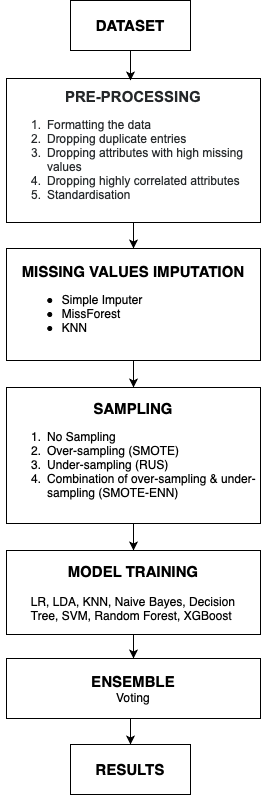
\includegraphics[width=.75\columnwidth]{Pipeline.png}
\caption{\label{fig::pipeline} Model Pipeline}
\end{figure}

\subsection{Pre-processing}
\label{sec::pipe_preprocessing}
The following tasks were performed as part of pre-processing:
\begin{itemize}
    \item The data was converted into a \texttt{.csv} format so that data analysis and training could be performed with ease.
    \item The dataset contained duplicate entries. Such entries were dropped.
    \item \texttt{Attr37} had over 40\% of the values missing and hence, was dropped. (Section \ref{sec::missing_vals}.
    \item In some cases, a pair of attributes in the dataset were highly correlated with each other (Section \ref{sec::correlation}). In such cases, the attributes with higher number of missing values were dropped. The list of attributes dropped are:
    \begin{quote}
        \{Attr3, Attr4, Attr6, Attr7, Attr15, Attr19, Attr32, Attr38, Attr43, Attr44, Attr49, Attr51, Attr60, Attr62\}
    \end{quote}
    \item Some models required the data to be standardised (removing the mean and scaling to unit variance).
\end{itemize}


\subsection{Missing values imputation}
\label{sec::pipe_missing_vals}
To tackle the missing values problem (Section \ref{sec::missing_vals}), the following techniques were studied:

\begin{itemize}
    \item \textbf{Simple Imputer}: Missing values are imputed with mean of each column in which the missing values are located.
    \item \textbf{MissForest Imputer}: Missing values are imputed using Random Forests in an iterative fashion \cite{Stekhoven_2011}.
    % Initially, the imputer begins imputing missing values of the column with the largest number of missing values (\textit{candidate} column). The first step involves filling any missing values of the remaining, \textit{non-candidate}, columns with an initial guess, which is the column mean. After that, the imputer fits a random forest model with the candidate column as the outcome variable and the remaining columns as the predictors over all rows where the candidate column values are not missing. After the fit, the missing rows of the candidate column are imputed using the prediction from the fitted Random Forest. The rows of the non-candidate columns act as the input data for the fitted model. Following this, the imputer moves on to the next candidate column with the second largest number of missing values from among the non-candidate columns in the first round. The process repeats itself for each column with a missing value, possibly over multiple iterations or epochs for each column, until the stopping criterion is met. The process is continued until the stopping criterion is reached, which is governed by the "difference" between the imputed arrays over successive iterations. 
    \item \textbf{KNN Imputer}: Missing values are imputed using k-Nearest Neighbors approach \cite{mani2003knn}.
\end{itemize}


\subsection{Sampling}
\label{sec::pipe_sampling}
To tackle the imbalance in class distributions (Section \ref{sec::imbalance}), over-sampling, under-sampling or a combination of both were performed and a comparative study was performed on the performance, along with the case where no sampling was performed.


\begin{itemize}
    \item \textbf{Over-sampling}: Synthetic Minority Oversampling Technique (SMOTE) \cite{Chawla_2002}
    \item \textbf{Under-sampling}:  Random Under-Sampling of majority class (RUS)
    \item \textbf{Over-sampling and Under-sampling}: combined over-sampling and under-sampling using SMOTE and Edited Nearest Neighbours (SMOTE-ENN)  \cite{Stekhoven_2011}.
    
\end{itemize}


\subsection{Modelling}
\label{sec::pipe_models}
The goal of the experiment was to identify the best classification model in terms of F1-score. We took under consideration the following classification methods:

\begin{itemize}
    \item \textbf{LR}: Logistic Regression 
    \item \textbf{LDA}: Linear Discriminant Analysis \cite{lda}
    \item \textbf{KNN-5}: k-Nearest Neighbours (with 5 neighbours) \cite{knn}
    \item \textbf{KNN-10}: k-Nearest Neighbours (with 10 neighbours)
    \item \textbf{GNB}: Gaussian Naive Bayes
    \item \textbf{DT}: Decision Tree
    \item \textbf{SVC}: Support Vector machine Classifier \cite{svc}
    \item \textbf{RFC}: Random Forest Classifier \cite{rf}
    \item \textbf{XGB}: eXtreme Gradient Boosting \cite{xgboost}
\end{itemize}

\subsubsection{Voting}
The top performing models were combined to build an ensemble model, in which a majority vote (\textit{hard} voting) would be used to predict the class labels. The aim is to balance out the individual weaknesses of each model.

Based on the results, we chose \textbf{LR}, \textbf{DT}, \textbf{RFC}, \textbf{XGB} with individual weights as $1$ and \textbf{KNN-10}, \textbf{SVC} with weights $0.5$ each in the voting to build a "Voting" Classifier.


\section{Experiment}

\subsection{Settings}

\begin{itemize}
    \item The models were implemented\footnote{Code available at \vargithubrepo} in Python using Scikit-learn \cite{scikit-learn}. MissingPy and Imbalanced-learn \cite{imb-learn} were used for imputing missing values and balancing classes in the dataset. xgboost package \cite{xgboost} was used to train XGBoost model (to leverage concurrency).  Matplotlib \cite{matplotlib} was used to plot graphs and Pandas \cite{pandas1,pandas2} was used for data analysis.
    
    \item Pre-processing as mentioned in Section \ref{sec::pipe_preprocessing} were performed.
    
    \item The \texttt{random\_state} was set to \varrandomstate wherever possible.
    
    \item The dataset was split into train-test sets using \texttt{ sklearn.model\_selection.train\_ test\_split()} with \texttt{test\_split} set to \varsplit.
    
    \item The experiment was conducted for each of the following 12 combinations of missing value imputation and sampling techniques (as mentioned in Section \ref{sec::methodology}) for each year:
        \begin{enumerate}
            \item \textbf{Simple} imputation with \textbf{No} sampling
        \item \textbf{Simple} imputation with \textbf{SMOTE} sampling
        \item \textbf{Simple} imputation with \textbf{RUS} sampling
        \item \textbf{Simple} imputation with \textbf{SMOTE-ENN} sampling
        \item \textbf{MissForest} imputation with \textbf{No} sampling
        \item \textbf{MissForest} imputation with \textbf{SMOTE} sampling
        \item \textbf{MissForest} imputation with \textbf{RUS} sampling
        \item \textbf{MissForest} imputation with \textbf{SMOTE-ENN} sampling
        \item \textbf{KNN} imputation with \textbf{No} sampling
        \item \textbf{KNN} imputation with \textbf{SMOTE} sampling
        \item \textbf{KNN} imputation with \textbf{RUS} sampling
        \item \textbf{KNN} imputation with \textbf{SMOTE-ENN} sampling
        \end{enumerate}
        
    \item The sampling was performed only on the train set. However, imputation had to be carried out in both train and test sets.
    
    \item The desired ratio of the number of samples in the minority class over the number of samples in the majority class after resampling is set to \vasamplingstrategy.
    
    \item Each model was tuned by performing exhaustive search over list of parameter values and fitted with \varcrossval-fold cross validation with \varcrossvalmetric as validation metric to obtained the best model. The list of parameters were chosen based on heuristics, considering the computational costs.
    % The list of parameters used and the best parameters obtained are enclosed in Appendix \ref{app::params}.
    
    %\item 


\end{itemize}
%%%%%%%%%%%% complete this
\subsection{Results}
\label{sec:results}
We use the following notations to define the performance metrics used in this report:
\begin{itemize}
    \item \textbf{TP} (True Positive): Model predicts Positive and it is actually Positive.
    \item \textbf{FP} (False Positive): Model predicts Positive but it is actually Negative.
    \item \textbf{FN} (False Negative): Model predicts Negative but it is actually Positive.
    \item \textbf{TN} (True Negative): Model predicts Negative and it is actually Negative.
\end{itemize}


\noindent Now, we define the performance metrics of our interest.
\begin{table}[htpb]
\centering
\begin{tabular}{lcl}
Accuracy \textit{(Acc)} & = & $\frac{TP + TN}{TP + FP + FN + TN}$ \\
~ & ~ & ~ \\
Precision \textit{(Prec)} & = & $\frac{TP}{TP + FP}$ \\
~ & ~ & ~ \\
Recall \textit{(Rec)} & = & $\frac{TP}{TP + FN}$ \\
~ & ~ & ~ \\
F1-Score \textit{(F1)} & = & $\frac{2 \times \text{Precision} \times
\text{Recall}}{\text{Precision}+\text{Recall}}$ \\
\end{tabular}
\end{table}

\begin{table*}[htbp]
\centering
\begin{tabular}[htbp]{r|cc|c|cccc}
     \textbf{Year} & \textbf{Imputer} & \textbf{Sampling} &\textbf{Model} & \textbf{Acc} & \textbf{Prec} & \textbf{Rec} &\textbf{F1}  \\
     \hline
     1 & Simple & SMOTE & XGBoost & 0.98 & 0.69 & 0.66 & 0.68 \\
     2 & Simple & None & XGBoost & 0.97 & 0.97 & 0.38 & 0.54 \\
     3 & Simple & SMOTE & XGBoost & 0.96 & 0.67 & 0.53 & 0.60 \\
     4 & Simple & SMOTE & XGBoost & 0.96 & 0.63 & 0.59 & 0.61 \\
     5 & Simple & SMOTE & XGBoost & 0.95 & 0.63 & 0.66 & 0.64 \\
\end{tabular}
\caption{\label{tab::best_results} Best results in each year}
\end{table*}


We list the model and the setting which gave the best results for each year in Table \ref{tab::best_results} and enclose the complete results obtained for each settings for each year in Table \ref{tab::results}.


\subsection{Analysis}
From the results in Table \ref{tab::best_results} and Table \ref{tab::results}, the following observations can be drawn:
\begin{itemize}
    \item XGBoost gave the best results, in terms of F1-score.
    \item The performance of the models had improved when over-sampling (specifically SMOTE) was used, in general.
    \item A surprising result was that Simple Imputation outperformed MissForest and KNN Imputation techniques, even though the latter methods are relatively more sophisticated and computationally expensive. 
    \item Both over-sampling and under-sampling (including combination of both) improved the recall, while the precision dropped. This can be reasoned by the fact that the sampling techniques increase the percentage of examples positive labels (\textit{minority} class) in the dataset. 
    
    
\end{itemize}


\section{Other Approaches}
Since many attributes had high correlation values with each other, we were motivated to use Dimensionality Reduction for the data-set, Principal Component Analysis (PCA) \cite{PCA:12} in particular. We reduced the dimension of the dataset to 20 and experimented with different sampling techniques and Simple Imputation.
%Table \ref{tab::pca_results} contains the results of the experiment. 
However, we observed that the results did not improve significantly with PCA (Table \ref{tab::pca_results}).



\section{Conclusion}
In this project, we surveyed various missing value imputation and sampling techniques and conducted a comparative study for bankruptcy prediction task. The performance of the models had improved significantly with the application of SMOTE (Table  \ref{tab::best_results} and Table \ref{tab::results}). \newcite{ren_2020} conducted the experiment for Year 5 without sampling and obtained a recall of 56\%. In our case, the best model for Year 5 had a recall of 66\% (and a F1-score of 64\%). Moreover, the accuracy values of the best models obtained were over 95\% which were similar to accuracy values obtained by \newcite{zikeba2016ensemble}. However, in our case, the model had learnt to predict companies that actually go "\textit{bankrupt}" (as the F1-scores were above 60\% on average); however no such conclusion can be drawn from the models proposed by \newcite{zikeba2016ensemble} as the F1-scores were not reported and owing to the high class imbalance, a model with high bias towards the class "\textit{not bankrupt}" could also have similar accuracy values (as discussed in Section \ref{sec::motivation}).


% en and Weiss (2020) trained some ML models for bankruptcy, including the XGBoost model by Zieba et al. (2016), and observed that the best recall value achieved was approx. 58%​
%They argued "the biggest issue with the results is that only 56% of the bankrupted companies are identified but given the relatively severe level of class imbalance (1:13.5), the results are non


%%% \section*{Acknowledgments}

%%% The acknowledgments should go immediately before the references. Do not number the acknowledgments section.
%% Do not include this section when submitting your paper for review.


\bibliography{bibs/main,bibs/py,bibs/models}
\bibliographystyle{acl_natbib}

\appendix

% \section{Complete Results}
\begin{table*}
% \ContinuedFloat
\begin{narrow}{-1cm}{-1cm}
\begin{subtable}[t]{2.05\columnwidth}
    \centering
    \begin{tabular}{l|r|c|cccccccccc}
       Imputer & Sampling & Metric & LR & LDA & KNN-5 & KNN-10 & GNB & DT & SVC & RFC & XGB & Voting \\
        \hline \hline
                        
        Simple & None & Acc & 0.96 & 0.96 & 0.96 & 0.96 & 0.07 & 0.98 & 0.96 & 0.98 & 0.98 & 0.98 \\
        ~ & ~ & Prec & 0.65 & 0.00 & 0.33 & 0.00 & 0.04 & 0.81 & 0.00 & 0.87 & 0.95 & 0.97 \\
        ~ & ~ & Rec & 0.19 & 0.00 & 0.01 & 0.00 & 0.99 & 0.56 & 0.00 & 0.50 & 0.54 & 0.50 \\
        ~ & ~ & F1 & 0.30 & 0.00 & 0.03 & 0.00 & 0.08 & 0.66 & 0.00 & 0.64 & 0.69 & 0.66 \\
        \cline{2-13}
        ~ & SMOTE & Acc & 0.87 & 0.94 & 0.84 & 0.85 & 0.06 & 0.85 & 0.90 & 0.98 & \textbf{0.98} & 0.98 \\
        ~ & ~ & Prec & 0.15 & 0.15 & 0.10 & 0.13 & 0.04 & 0.18 & 0.23 & 0.77 & \textbf{0.69} & 0.81 \\
        ~ & ~ & Rec & 0.47 & 0.09 & 0.40 & 0.53 & 1.00 & 0.76 & 0.60 & 0.53 & \textbf{0.66} & 0.62 \\
        ~ & ~ & F1 & 0.23 & 0.11 & 0.16 & 0.21 & 0.08 & 0.29 & 0.33 & 0.63 & \textbf{0.68} & 0.70 \\
        \cline{2-13}
        ~ & RUS & Acc & 0.87 & 0.87 & 0.81 & 0.85 & 0.66 & 0.85 & 0.92 & 0.91 & 0.92 & 0.94 \\
        ~ & ~ & Prec & 0.15 & 0.12 & 0.10 & 0.11 & 0.06 & 0.19 & 0.10 & 0.27 & 0.29 & 0.35 \\
        ~ & ~ & Rec & 0.51 & 0.34 & 0.47 & 0.38 & 0.49 & 0.84 & 0.12 & 0.74 & 0.81 & 0.76 \\
        ~ & ~ & F1 & 0.23 & 0.17 & 0.16 & 0.17 & 0.10 & 0.31 & 0.11 & 0.40 & 0.43 & 0.48 \\
        \cline{2-13}
        ~ & SMOTE- & Acc & 0.81 & 0.88 & 0.80 & 0.78 & 0.09 & 0.95 & 0.79 & 0.97 & 0.97 & 0.97 \\
        ~ & ENN & Prec & 0.13 & 0.11 & 0.11 & 0.10 & 0.04 & 0.39 & 0.10 & 0.67 & 0.63 & 0.61 \\
        ~ & ~ & Rec & 0.69 & 0.31 & 0.56 & 0.54 & 0.99 & 0.65 & 0.54 & 0.54 & 0.71 & 0.68 \\
        ~ & ~ & F1 & 0.22 & 0.16 & 0.18 & 0.16 & 0.08 & 0.48 & 0.17 & 0.60 & 0.67 & 0.64 \\
        \hline\hline
        
        MissForest & None & Acc & 0.96 & 0.96 & 0.96 & 0.96 & 0.95 & 0.94 & 0.96 & 0.96 & 0.96 & 0.96 \\
        ~ & ~ & Prec & 0.17 & 0.00 & 0.00 & 0.00 & 0.09 & 0.22 & 0.00 & 0.00 & 0.80 & 0.00 \\
        ~ & ~ & Rec & 0.01 & 0.00 & 0.00 & 0.00 & 0.03 & 0.21 & 0.00 & 0.00 & 0.06 & 0.00 \\
        ~ & ~ & F1 & 0.03 & 0.00 & 0.00 & 0.00 & 0.04 & 0.21 & 0.00 & 0.00 & 0.11 & 0.00 \\
        \cline{2-13}
        ~ & SMOTE & Acc & 0.87 & 0.94 & 0.82 & 0.82 & 0.07 & 0.84 & 0.93 & 0.95 & 0.94 & 0.95 \\
        ~ & ~ & Prec & 0.13 & 0.10 & 0.11 & 0.10 & 0.04 & 0.11 & 0.18 & 0.32 & 0.31 & 0.33 \\
        ~ & ~ & Rec & 0.40 & 0.06 & 0.50 & 0.46 & 0.99 & 0.44 & 0.21 & 0.28 & 0.40 & 0.37 \\
        ~ & ~ & F1 & 0.20 & 0.07 & 0.18 & 0.17 & 0.08 & 0.17 & 0.19 & 0.30 & 0.35 & 0.35 \\
        \cline{2-13}
        ~ & RUS & Acc & 0.92 & 0.87 & 0.79 & 0.87 & 0.91 & 0.80 & 0.95 & 0.86 & 0.85 & 0.91 \\
        ~ & ~ & Prec & 0.16 & 0.12 & 0.09 & 0.07 & 0.04 & 0.08 & 0.09 & 0.16 & 0.16 & 0.17 \\
        ~ & ~ & Rec & 0.22 & 0.37 & 0.47 & 0.21 & 0.06 & 0.41 & 0.04 & 0.57 & 0.69 & 0.34 \\
        ~ & ~ & F1 & 0.18 & 0.18 & 0.15 & 0.11 & 0.05 & 0.14 & 0.06 & 0.25 & 0.26 & 0.23 \\
        \cline{2-13}
        ~ & SMOTE- & Acc & 0.76 & 0.84 & 0.77 & 0.76 & 0.10 & 0.84 & 0.85 & 0.92 & 0.89 & 0.89 \\
        ~ & ENN & Prec & 0.12 & 0.08 & 0.09 & 0.09 & 0.04 & 0.12 & 0.12 & 0.22 & 0.18 & 0.18 \\
        ~ & ~ & Rec & 0.78 & 0.29 & 0.54 & 0.56 & 0.93 & 0.51 & 0.43 & 0.37 & 0.51 & 0.53 \\
        ~ & ~ & F1 & 0.20 & 0.13 & 0.16 & 0.15 & 0.07 & 0.20 & 0.18 & 0.27 & 0.27 & 0.27 \\
        \hline\hline
        
        KNN & None & Acc & 0.96 & 0.96 & 0.96 & 0.96 & 0.07 & 0.94 & 0.96 & 0.96 & 0.96 & 0.96 \\
        ~ & ~ & Prec & 0.00 & 0.00 & 0.17 & 0.00 & 0.04 & 0.25 & 0.00 & 0.17 & 0.77 & 0.00 \\
        ~ & ~ & Rec & 0.00 & 0.00 & 0.01 & 0.00 & 0.99 & 0.25 & 0.00 & 0.01 & 0.15 & 0.00 \\
        ~ & ~ & F1 & 0.00 & 0.00 & 0.03 & 0.00 & 0.08 & 0.25 & 0.00 & 0.03 & 0.25 & 0.00 \\
        \cline{2-13}
        ~ & SMOTE & Acc & 0.87 & 0.94 & 0.83 & 0.83 & 0.09 & 0.89 & 0.93 & 0.94 & 0.95 & 0.95 \\
        ~ & ~ & Prec & 0.13 & 0.11 & 0.10 & 0.11 & 0.04 & 0.15 & 0.18 & 0.26 & 0.39 & 0.34 \\
        ~ & ~ & Rec & 0.41 & 0.07 & 0.40 & 0.50 & 0.96 & 0.40 & 0.25 & 0.32 & 0.46 & 0.24 \\
        ~ & ~ & F1 & 0.20 & 0.09 & 0.15 & 0.18 & 0.08 & 0.22 & 0.21 & 0.29 & 0.42 & 0.28 \\
        \cline{2-13}
        ~ & RUS & Acc & 0.91 & 0.86 & 0.79 & 0.82 & 0.12 & 0.84 & 0.92 & 0.87 & 0.86 & 0.91 \\
        ~ & ~ & Prec & 0.15 & 0.12 & 0.09 & 0.09 & 0.04 & 0.12 & 0.10 & 0.18 & 0.17 & 0.18 \\
        ~ & ~ & Rec & 0.28 & 0.38 & 0.47 & 0.38 & 1.00 & 0.47 & 0.12 & 0.60 & 0.68 & 0.37 \\
        ~ & ~ & F1 & 0.20 & 0.18 & 0.15 & 0.14 & 0.08 & 0.19 & 0.11 & 0.27 & 0.27 & 0.24 \\
        \cline{2-13}
        ~ & SMOTE- & Acc & 0.82 & 0.84 & 0.78 & 0.76 & 0.09 & 0.77 & 0.78 & 0.90 & 0.94 & 0.92 \\
        ~ & ENN & Prec & 0.10 & 0.11 & 0.10 & 0.09 & 0.04 & 0.10 & 0.10 & 0.17 & 0.33 & 0.21 \\
        ~ & ~ & Rec & 0.46 & 0.44 & 0.56 & 0.57 & 0.96 & 0.63 & 0.57 & 0.44 & 0.57 & 0.34 \\
        ~ & ~ & F1 & 0.16 & 0.18 & 0.17 & 0.16 & 0.08 & 0.18 & 0.17 & 0.25 & 0.42 & 0.26 \\

         \hline \hline
    \end{tabular}
    \caption{\label{tab::results_y1} Year 1}
    
   
\end{subtable}

\end{narrow}
\end{table*} 






\begin{table*}
\ContinuedFloat
\begin{narrow}{-1cm}{-1cm}
\begin{subtable}[t]{2.05\columnwidth}
    \centering
    \begin{tabular}{l|r|c|cccccccccc}
       Imputer & Sampling & Metric & LR & LDA & KNN-5 & KNN-10 & GNB & DT & SVC & RFC & XGB & Voting \\
        \hline \hline
                
        Simple & None & Acc & 0.96 & 0.96 & 0.96 & 0.96 & 0.06 & 0.97 & 0.96 & 0.97 & \textbf{0.97} & 0.97 \\
        ~ & ~ & Prec & 0.33 & 0.40 & 0.00 & 0.00 & 0.04 & 0.71 & 0.00 & 0.85 & \textbf{0.97} & 0.95 \\
        ~ & ~ & Rec & 0.02 & 0.02 & 0.00 & 0.00 & 0.93 & 0.25 & 0.00 & 0.22 & \textbf{0.38} & 0.20 \\
        ~ & ~ & F1 & 0.04 & 0.04 & 0.00 & 0.00 & 0.07 & 0.37 & 0.00 & 0.35 & \textbf{0.54} & 0.33 \\
        \cline{2-13}
        ~ & SMOTE & Acc & 0.86 & 0.93 & 0.81 & 0.80 & 0.08 & 0.92 & 0.86 & 0.97 & 0.97 & 0.97 \\
        ~ & ~ & Prec & 0.12 & 0.07 & 0.08 & 0.07 & 0.04 & 0.20 & 0.13 & 0.74 & 0.67 & 0.67 \\
        ~ & ~ & Rec & 0.40 & 0.06 & 0.36 & 0.34 & 0.90 & 0.36 & 0.41 & 0.28 & 0.39 & 0.34 \\
        ~ & ~ & F1 & 0.19 & 0.06 & 0.13 & 0.12 & 0.07 & 0.26 & 0.19 & 0.41 & 0.49 & 0.45 \\
        \cline{2-13}
        ~ & RUS & Acc & 0.82 & 0.84 & 0.73 & 0.81 & 0.88 & 0.86 & 0.87 & 0.87 & 0.88 & 0.91 \\
        ~ & ~ & Prec & 0.10 & 0.08 & 0.08 & 0.08 & 0.06 & 0.16 & 0.07 & 0.18 & 0.21 & 0.24 \\
        ~ & ~ & Rec & 0.46 & 0.28 & 0.53 & 0.36 & 0.14 & 0.60 & 0.20 & 0.66 & 0.69 & 0.62 \\
        ~ & ~ & F1 & 0.17 & 0.12 & 0.13 & 0.13 & 0.09 & 0.25 & 0.11 & 0.28 & 0.32 & 0.35 \\
        \cline{2-13}
        ~ & SMOTE- & Acc & 0.72 & 0.83 & 0.74 & 0.73 & 0.05 & 0.88 & 0.78 & 0.96 & 0.96 & 0.95 \\
        ~ & ENN & Prec & 0.08 & 0.07 & 0.07 & 0.07 & 0.04 & 0.15 & 0.09 & 0.52 & 0.50 & 0.42 \\
        ~ & ~ & Rec & 0.55 & 0.28 & 0.43 & 0.48 & 0.99 & 0.41 & 0.51 & 0.26 & 0.39 & 0.45 \\
        ~ & ~ & F1 & 0.13 & 0.11 & 0.12 & 0.12 & 0.08 & 0.21 & 0.15 & 0.35 & 0.44 & 0.43 \\
        \hline\hline
        
        MissForest & None & Acc & 0.96 & 0.96 & 0.96 & 0.96 & 0.08 & 0.95 & 0.96 & 0.96 & 0.97 & 0.96 \\
        ~ & ~ & Prec & 0.33 & 0.25 & 0.00 & 0.00 & 0.04 & 0.37 & 0.00 & 0.12 & 0.80 & 1.00 \\
        ~ & ~ & Rec & 0.02 & 0.04 & 0.00 & 0.00 & 0.89 & 0.21 & 0.00 & 0.01 & 0.16 & 0.01 \\
        ~ & ~ & F1 & 0.04 & 0.07 & 0.00 & 0.00 & 0.07 & 0.27 & 0.00 & 0.02 & 0.27 & 0.02 \\
        \cline{2-13}
        ~ & SMOTE & Acc & 0.83 & 0.93 & 0.80 & 0.79 & 0.09 & 0.83 & 0.83 & 0.92 & 0.96 & 0.94 \\
        ~ & ~ & Prec & 0.10 & 0.09 & 0.08 & 0.07 & 0.04 & 0.11 & 0.10 & 0.20 & 0.45 & 0.25 \\
        ~ & ~ & Rec & 0.40 & 0.08 & 0.38 & 0.35 & 0.89 & 0.46 & 0.43 & 0.31 & 0.34 & 0.28 \\
        ~ & ~ & F1 & 0.16 & 0.09 & 0.13 & 0.11 & 0.07 & 0.18 & 0.16 & 0.24 & 0.39 & 0.26 \\
        \cline{2-13}
        ~ & RUS & Acc & 0.82 & 0.86 & 0.72 & 0.80 & 0.92 & 0.77 & 0.86 & 0.83 & 0.84 & 0.87 \\
        ~ & ~ & Prec & 0.08 & 0.08 & 0.07 & 0.06 & 0.06 & 0.09 & 0.06 & 0.14 & 0.15 & 0.14 \\
        ~ & ~ & Rec & 0.33 & 0.24 & 0.50 & 0.27 & 0.07 & 0.52 & 0.18 & 0.62 & 0.64 & 0.45 \\
        ~ & ~ & F1 & 0.13 & 0.12 & 0.12 & 0.10 & 0.07 & 0.15 & 0.09 & 0.22 & 0.24 & 0.22 \\
        \cline{2-13}
        ~ & SMOTE- & Acc & 0.71 & 0.83 & 0.73 & 0.72 & 0.09 & 0.82 & 0.76 & 0.88 & 0.93 & 0.88 \\
        ~ & ENN & Prec & 0.07 & 0.07 & 0.07 & 0.07 & 0.04 & 0.09 & 0.08 & 0.14 & 0.27 & 0.15 \\
        ~ & ~ & Rec & 0.55 & 0.24 & 0.47 & 0.46 & 0.89 & 0.40 & 0.50 & 0.37 & 0.37 & 0.45 \\
        ~ & ~ & F1 & 0.13 & 0.10 & 0.12 & 0.12 & 0.07 & 0.15 & 0.14 & 0.20 & 0.31 & 0.23 \\
        \hline\hline
        
        
        KNN & None & Acc & 0.96 & 0.96 & 0.96 & 0.96 & 0.07 & 0.94 & 0.96 & 0.96 & 0.96 & 0.96 \\
        ~ & ~ & Prec & 0.33 & 0.40 & 0.00 & 0.00 & 0.04 & 0.19 & 0.00 & 0.12 & 0.73 & 0.33 \\
        ~ & ~ & Rec & 0.02 & 0.02 & 0.00 & 0.00 & 0.91 & 0.18 & 0.00 & 0.01 & 0.16 & 0.01 \\
        ~ & ~ & F1 & 0.04 & 0.04 & 0.00 & 0.00 & 0.07 & 0.18 & 0.00 & 0.02 & 0.26 & 0.02 \\
        \cline{2-13}
        ~ & SMOTE & Acc & 0.85 & 0.93 & 0.80 & 0.78 & 0.08 & 0.86 & 0.83 & 0.93 & 0.92 & 0.93 \\
        ~ & ~ & Prec & 0.12 & 0.07 & 0.08 & 0.06 & 0.04 & 0.12 & 0.10 & 0.19 & 0.21 & 0.23 \\
        ~ & ~ & Rec & 0.42 & 0.06 & 0.36 & 0.32 & 0.91 & 0.39 & 0.40 & 0.27 & 0.35 & 0.31 \\
        ~ & ~ & F1 & 0.18 & 0.06 & 0.12 & 0.10 & 0.07 & 0.19 & 0.16 & 0.22 & 0.27 & 0.26 \\
        \cline{2-13}
        ~ & RUS & Acc & 0.81 & 0.85 & 0.71 & 0.79 & 0.89 & 0.82 & 0.86 & 0.82 & 0.82 & 0.88 \\
        ~ & ~ & Prec & 0.10 & 0.09 & 0.07 & 0.06 & 0.06 & 0.11 & 0.07 & 0.12 & 0.12 & 0.15 \\
        ~ & ~ & Rec & 0.44 & 0.30 & 0.52 & 0.31 & 0.13 & 0.49 & 0.19 & 0.59 & 0.58 & 0.45 \\
        ~ & ~ & F1 & 0.16 & 0.14 & 0.12 & 0.11 & 0.08 & 0.18 & 0.10 & 0.20 & 0.20 & 0.23 \\
        \cline{2-13}
        ~ & SMOTE- & Acc & 0.70 & 0.82 & 0.73 & 0.72 & 0.05 & 0.67 & 0.75 & 0.86 & 0.93 & 0.88 \\
        ~ & ENN & Prec & 0.08 & 0.07 & 0.06 & 0.07 & 0.04 & 0.07 & 0.08 & 0.12 & 0.24 & 0.14 \\
        ~ & ~ & Rec & 0.59 & 0.28 & 0.43 & 0.46 & 0.99 & 0.56 & 0.51 & 0.42 & 0.37 & 0.40 \\
        ~ & ~ & F1 & 0.14 & 0.11 & 0.11 & 0.11 & 0.08 & 0.12 & 0.14 & 0.19 & 0.29 & 0.20 \\
         \hline \hline
         
    \end{tabular}
    \caption{\label{tab::results_y2} Year 2}
    
   
\end{subtable}

\end{narrow}
\end{table*} 






\begin{table*}
\ContinuedFloat
\begin{narrow}{-1cm}{-1cm}
\begin{subtable}[t]{2.05\columnwidth}
    \centering
    \begin{tabular}{l|r|c|cccccccccc}
       Imputer & Sampling & Metric & LR & LDA & KNN-5 & KNN-10 & GNB & DT & SVC & RFC & XGB & Voting \\
        \hline \hline
        
        Simple & None & Acc & 0.95 & 0.95 & 0.94 & 0.95 & 0.07 & 0.96 & 0.95 & 0.96 & 0.97 & 0.97 \\
        ~ & ~ & Prec & 0.06 & 0.00 & 0.00 & 0.00 & 0.05 & 0.66 & 0.00 & 0.79 & 0.87 & 1.00 \\
        ~ & ~ & Rec & 0.01 & 0.00 & 0.00 & 0.00 & 0.99 & 0.42 & 0.00 & 0.34 & 0.45 & 0.31 \\
        ~ & ~ & F1 & 0.01 & 0.00 & 0.00 & 0.00 & 0.09 & 0.51 & 0.00 & 0.48 & 0.59 & 0.47 \\
        \cline{2-13}
        ~ & SMOTE & Acc & 0.85 & 0.92 & 0.81 & 0.80 & 0.06 & 0.93 & 0.86 & 0.96 & \textbf{0.96} & 0.96 \\
        ~ & ~ & Prec & 0.16 & 0.15 & 0.11 & 0.10 & 0.05 & 0.35 & 0.18 & 0.54 & \textbf{0.67} & 0.62 \\
        ~ & ~ & Rec & 0.49 & 0.15 & 0.40 & 0.43 & 0.99 & 0.51 & 0.52 & 0.45 & \textbf{0.53} & 0.45 \\
        ~ & ~ & F1 & 0.24 & 0.15 & 0.17 & 0.17 & 0.09 & 0.42 & 0.26 & 0.49 & \textbf{0.60} & 0.52 \\
        \cline{2-13}
        ~ & RUS & Acc & 0.88 & 0.87 & 0.77 & 0.80 & 0.12 & 0.92 & 0.85 & 0.89 & 0.89 & 0.93 \\
        ~ & ~ & Prec & 0.23 & 0.14 & 0.10 & 0.11 & 0.05 & 0.32 & 0.11 & 0.26 & 0.29 & 0.37 \\
        ~ & ~ & Rec & 0.64 & 0.33 & 0.49 & 0.46 & 0.96 & 0.57 & 0.33 & 0.75 & 0.82 & 0.68 \\
        ~ & ~ & F1 & 0.34 & 0.19 & 0.17 & 0.18 & 0.09 & 0.41 & 0.17 & 0.39 & 0.42 & 0.48 \\
        \cline{2-13}
        ~ & SMOTE- & Acc & 0.74 & 0.83 & 0.74 & 0.72 & 0.11 & 0.89 & 0.74 & 0.95 & 0.96 & 0.94 \\
        ~ & ENN & Prec & 0.12 & 0.12 & 0.09 & 0.09 & 0.05 & 0.23 & 0.12 & 0.44 & 0.54 & 0.39 \\
        ~ & ~ & Rec & 0.71 & 0.41 & 0.49 & 0.57 & 0.94 & 0.61 & 0.68 & 0.47 & 0.59 & 0.62 \\
        ~ & ~ & F1 & 0.20 & 0.18 & 0.15 & 0.16 & 0.09 & 0.33 & 0.20 & 0.45 & 0.57 & 0.48 \\
        \hline\hline
        
        MissForest & None & Acc & 0.95 & 0.95 & 0.95 & 0.95 & 0.08 & 0.93 & 0.95 & 0.95 & 0.96 & 0.95 \\
        ~ & ~ & Prec & 0.05 & 0.05 & 0.00 & 0.00 & 0.05 & 0.20 & 0.00 & 0.08 & 0.82 & 0.50 \\
        ~ & ~ & Rec & 0.01 & 0.01 & 0.00 & 0.00 & 1.00 & 0.14 & 0.00 & 0.01 & 0.15 & 0.01 \\
        ~ & ~ & F1 & 0.01 & 0.01 & 0.00 & 0.00 & 0.09 & 0.17 & 0.00 & 0.01 & 0.25 & 0.02 \\
        \cline{2-13}
        ~ & SMOTE & Acc & 0.86 & 0.93 & 0.81 & 0.79 & 0.06 & 0.79 & 0.86 & 0.92 & 0.95 & 0.93 \\
        ~ & ~ & Prec & 0.15 & 0.11 & 0.10 & 0.10 & 0.05 & 0.11 & 0.11 & 0.28 & 0.46 & 0.26 \\
        ~ & ~ & Rec & 0.45 & 0.08 & 0.37 & 0.44 & 0.99 & 0.50 & 0.29 & 0.40 & 0.30 & 0.33 \\
        ~ & ~ & F1 & 0.23 & 0.09 & 0.15 & 0.17 & 0.09 & 0.19 & 0.16 & 0.33 & 0.36 & 0.29 \\
        \cline{2-13}
        ~ & RUS & Acc & 0.87 & 0.89 & 0.75 & 0.79 & 0.40 & 0.70 & 0.85 & 0.83 & 0.84 & 0.86 \\
        ~ & ~ & Prec & 0.14 & 0.10 & 0.09 & 0.10 & 0.06 & 0.10 & 0.11 & 0.16 & 0.18 & 0.20 \\
        ~ & ~ & Rec & 0.36 & 0.19 & 0.48 & 0.44 & 0.77 & 0.69 & 0.30 & 0.65 & 0.67 & 0.63 \\
        ~ & ~ & F1 & 0.21 & 0.13 & 0.16 & 0.16 & 0.11 & 0.18 & 0.16 & 0.26 & 0.29 & 0.30 \\
        \cline{2-13}
        ~ & SMOTE- & Acc & 0.76 & 0.86 & 0.74 & 0.72 & 0.12 & 0.82 & 0.77 & 0.88 & 0.94 & 0.88 \\
        ~ & ENN & Prec & 0.13 & 0.12 & 0.08 & 0.09 & 0.05 & 0.12 & 0.12 & 0.17 & 0.38 & 0.21 \\
        ~ & ~ & Rec & 0.69 & 0.33 & 0.46 & 0.50 & 0.98 & 0.44 & 0.63 & 0.37 & 0.42 & 0.54 \\
        ~ & ~ & F1 & 0.21 & 0.18 & 0.14 & 0.15 & 0.10 & 0.19 & 0.20 & 0.23 & 0.40 & 0.31 \\
        \hline\hline
        
        KNN & None & Acc & 0.95 & 0.95 & 0.94 & 0.95 & 0.07 & 0.94 & 0.95 & 0.95 & 0.96 & 0.95 \\
        ~ & ~ & Prec & 0.05 & 0.00 & 0.00 & 0.00 & 0.05 & 0.21 & 0.00 & 0.07 & 0.83 & 0.00 \\
        ~ & ~ & Rec & 0.01 & 0.00 & 0.00 & 0.00 & 0.99 & 0.14 & 0.00 & 0.01 & 0.12 & 0.00 \\
        ~ & ~ & F1 & 0.01 & 0.00 & 0.00 & 0.00 & 0.09 & 0.17 & 0.00 & 0.01 & 0.21 & 0.00 \\
        \cline{2-13}
        ~ & SMOTE & Acc & 0.85 & 0.92 & 0.80 & 0.78 & 0.06 & 0.85 & 0.85 & 0.91 & 0.95 & 0.92 \\
        ~ & ~ & Prec & 0.14 & 0.14 & 0.10 & 0.10 & 0.05 & 0.13 & 0.12 & 0.22 & 0.45 & 0.23 \\
        ~ & ~ & Rec & 0.44 & 0.14 & 0.40 & 0.44 & 0.99 & 0.35 & 0.37 & 0.33 & 0.37 & 0.26 \\
        ~ & ~ & F1 & 0.22 & 0.14 & 0.16 & 0.16 & 0.09 & 0.19 & 0.19 & 0.26 & 0.40 & 0.24 \\
        \cline{2-13}
        ~ & RUS & Acc & 0.85 & 0.88 & 0.76 & 0.79 & 0.10 & 0.82 & 0.85 & 0.80 & 0.83 & 0.84 \\
        ~ & ~ & Prec & 0.15 & 0.11 & 0.10 & 0.11 & 0.05 & 0.10 & 0.11 & 0.15 & 0.17 & 0.17 \\
        ~ & ~ & Rec & 0.46 & 0.22 & 0.50 & 0.46 & 0.97 & 0.34 & 0.33 & 0.66 & 0.70 & 0.58 \\
        ~ & ~ & F1 & 0.22 & 0.15 & 0.16 & 0.17 & 0.09 & 0.15 & 0.17 & 0.24 & 0.28 & 0.26 \\
        \cline{2-13}
        ~ & SMOTE- & Acc & 0.74 & 0.83 & 0.73 & 0.71 & 0.11 & 0.84 & 0.75 & 0.91 & 0.91 & 0.91 \\
        ~ & ENN & Prec & 0.12 & 0.12 & 0.09 & 0.09 & 0.05 & 0.13 & 0.12 & 0.21 & 0.28 & 0.21 \\
        ~ & ~ & Rec & 0.70 & 0.40 & 0.49 & 0.55 & 0.94 & 0.41 & 0.67 & 0.35 & 0.53 & 0.36 \\
        ~ & ~ & F1 & 0.20 & 0.18 & 0.14 & 0.15 & 0.09 & 0.20 & 0.20 & 0.27 & 0.36 & 0.27 \\

       \hline \hline
         
         
    \end{tabular}
    \caption{\label{tab::results_y3} Year 3}
    
   
\end{subtable}

\end{narrow}
\end{table*} 





\begin{table*}
\ContinuedFloat
\begin{narrow}{-1cm}{-1cm}
\begin{subtable}[t]{2.05\columnwidth}
    \centering
    \begin{tabular}{l|r|c|cccccccccc}
       Imputer & Sampling & Metric & LR & LDA & KNN-5 & KNN-10 & GNB & DT & SVC & RFC & XGB & Voting \\
        \hline \hline
        
        Simple & None & Acc & 0.94 & 0.94 & 0.95 & 0.94 & 0.10 & 0.95 & 0.95 & 0.96 & 0.97 & 0.96 \\
        ~ & ~ & Prec & 0.29 & 0.22 & 0.00 & 0.00 & 0.05 & 0.58 & 0.00 & 0.75 & 0.89 & 0.94 \\
        ~ & ~ & Rec & 0.03 & 0.03 & 0.00 & 0.00 & 0.94 & 0.33 & 0.00 & 0.23 & 0.45 & 0.23 \\
        ~ & ~ & F1 & 0.06 & 0.05 & 0.00 & 0.00 & 0.10 & 0.42 & 0.00 & 0.36 & 0.59 & 0.36 \\
        \cline{2-13}
        ~ & SMOTE & Acc & 0.88 & 0.91 & 0.81 & 0.81 & 0.08 & 0.88 & 0.89 & 0.93 & \textbf{0.96} & 0.95 \\
        ~ & ~ & Prec & 0.21 & 0.18 & 0.12 & 0.13 & 0.05 & 0.24 & 0.22 & 0.41 & \textbf{0.63} & 0.51 \\
        ~ & ~ & Rec & 0.45 & 0.20 & 0.41 & 0.43 & 0.95 & 0.58 & 0.46 & 0.52 & \textbf{0.59} & 0.52 \\
        ~ & ~ & F1 & 0.28 & 0.19 & 0.19 & 0.20 & 0.10 & 0.34 & 0.30 & 0.46 & \textbf{0.61} & 0.51 \\
        \cline{2-13}
        ~ & RUS & Acc & 0.86 & 0.88 & 0.80 & 0.83 & 0.90 & 0.86 & 0.90 & 0.86 & 0.90 & 0.90 \\
        ~ & ~ & Prec & 0.19 & 0.17 & 0.13 & 0.15 & 0.12 & 0.21 & 0.18 & 0.24 & 0.33 & 0.30 \\
        ~ & ~ & Rec & 0.53 & 0.33 & 0.48 & 0.45 & 0.14 & 0.59 & 0.25 & 0.73 & 0.82 & 0.66 \\
        ~ & ~ & F1 & 0.28 & 0.22 & 0.20 & 0.22 & 0.13 & 0.31 & 0.21 & 0.36 & 0.47 & 0.42 \\
        \cline{2-13}
        ~ & SMOTE- & Acc & 0.79 & 0.84 & 0.75 & 0.73 & 0.09 & 0.88 & 0.84 & 0.94 & 0.93 & 0.92 \\
        ~ & ENN & Prec & 0.14 & 0.16 & 0.12 & 0.11 & 0.05 & 0.25 & 0.16 & 0.44 & 0.42 & 0.36 \\
        ~ & ~ & Rec & 0.59 & 0.46 & 0.56 & 0.57 & 0.96 & 0.61 & 0.48 & 0.42 & 0.63 & 0.58 \\
        ~ & ~ & F1 & 0.23 & 0.24 & 0.19 & 0.18 & 0.10 & 0.35 & 0.25 & 0.43 & 0.51 & 0.45 \\
        \hline\hline

        MissForest & None & Acc & 0.95 & 0.94 & 0.94 & 0.95 & 0.13 & 0.92 & 0.95 & 0.95 & 0.95 & 0.95 \\
        ~ & ~ & Prec & 0.27 & 0.22 & 0.00 & 0.14 & 0.05 & 0.26 & 0.00 & 0.47 & 0.79 & 0.78 \\
        ~ & ~ & Rec & 0.02 & 0.03 & 0.00 & 0.01 & 0.90 & 0.23 & 0.00 & 0.06 & 0.17 & 0.05 \\
        ~ & ~ & F1 & 0.04 & 0.05 & 0.00 & 0.01 & 0.10 & 0.24 & 0.00 & 0.11 & 0.28 & 0.10 \\
        \cline{2-13}
        ~ & SMOTE & Acc & 0.84 & 0.88 & 0.81 & 0.82 & 0.12 & 0.86 & 0.89 & 0.92 & 0.94 & 0.93 \\
        ~ & ~ & Prec & 0.17 & 0.15 & 0.12 & 0.12 & 0.05 & 0.20 & 0.19 & 0.31 & 0.43 & 0.33 \\
        ~ & ~ & Rec & 0.50 & 0.27 & 0.41 & 0.41 & 0.87 & 0.57 & 0.33 & 0.45 & 0.45 & 0.34 \\
        ~ & ~ & F1 & 0.25 & 0.19 & 0.19 & 0.19 & 0.09 & 0.30 & 0.24 & 0.36 & 0.44 & 0.34 \\
        \cline{2-13}
        ~ & RUS & Acc & 0.82 & 0.84 & 0.80 & 0.88 & 0.87 & 0.81 & 0.86 & 0.84 & 0.85 & 0.88 \\
        ~ & ~ & Prec & 0.16 & 0.14 & 0.12 & 0.18 & 0.11 & 0.15 & 0.14 & 0.18 & 0.19 & 0.22 \\
        ~ & ~ & Rec & 0.54 & 0.38 & 0.46 & 0.37 & 0.22 & 0.56 & 0.34 & 0.59 & 0.61 & 0.54 \\
        ~ & ~ & F1 & 0.24 & 0.20 & 0.20 & 0.24 & 0.15 & 0.24 & 0.20 & 0.28 & 0.29 & 0.32 \\
        \cline{2-13}
        ~ & SMOTE- & Acc & 0.75 & 0.82 & 0.76 & 0.74 & 0.12 & 0.81 & 0.83 & 0.89 & 0.90 & 0.88 \\
        ~ & ENN & Prec & 0.13 & 0.14 & 0.11 & 0.11 & 0.05 & 0.16 & 0.15 & 0.23 & 0.29 & 0.21 \\
        ~ & ~ & Rec & 0.64 & 0.48 & 0.52 & 0.57 & 0.88 & 0.59 & 0.51 & 0.51 & 0.55 & 0.50 \\
        ~ & ~ & F1 & 0.22 & 0.22 & 0.19 & 0.19 & 0.09 & 0.25 & 0.23 & 0.32 & 0.38 & 0.30 \\
        \hline\hline

        KNN & None & Acc & 0.94 & 0.94 & 0.94 & 0.94 & 0.10 & 0.91 & 0.95 & 0.95 & 0.96 & 0.95 \\
        ~ & ~ & Prec & 0.31 & 0.22 & 0.00 & 0.00 & 0.05 & 0.19 & 0.00 & 0.47 & 0.92 & 0.80 \\
        ~ & ~ & Rec & 0.04 & 0.03 & 0.00 & 0.00 & 0.94 & 0.22 & 0.00 & 0.06 & 0.17 & 0.03 \\
        ~ & ~ & F1 & 0.07 & 0.05 & 0.00 & 0.00 & 0.10 & 0.20 & 0.00 & 0.11 & 0.29 & 0.06 \\
        \cline{2-13}
        ~ & SMOTE & Acc & 0.88 & 0.91 & 0.79 & 0.80 & 0.09 & 0.82 & 0.90 & 0.92 & 0.93 & 0.92 \\
        ~ & ~ & Prec & 0.20 & 0.18 & 0.11 & 0.11 & 0.05 & 0.14 & 0.20 & 0.31 & 0.38 & 0.30 \\
        ~ & ~ & Rec & 0.45 & 0.20 & 0.39 & 0.41 & 0.95 & 0.46 & 0.27 & 0.41 & 0.49 & 0.38 \\
        ~ & ~ & F1 & 0.28 & 0.19 & 0.17 & 0.18 & 0.10 & 0.22 & 0.23 & 0.35 & 0.43 & 0.33 \\
        \cline{2-13}
        ~ & RUS & Acc & 0.86 & 0.88 & 0.77 & 0.86 & 0.90 & 0.83 & 0.90 & 0.84 & 0.85 & 0.88 \\
        ~ & ~ & Prec & 0.18 & 0.16 & 0.11 & 0.15 & 0.12 & 0.16 & 0.19 & 0.18 & 0.20 & 0.22 \\
        ~ & ~ & Rec & 0.48 & 0.32 & 0.46 & 0.37 & 0.14 & 0.51 & 0.27 & 0.60 & 0.64 & 0.49 \\
        ~ & ~ & F1 & 0.26 & 0.21 & 0.17 & 0.22 & 0.13 & 0.24 & 0.22 & 0.28 & 0.30 & 0.30 \\
        \cline{2-13}
        ~ & SMOTE- & Acc & 0.80 & 0.84 & 0.73 & 0.71 & 0.09 & 0.79 & 0.81 & 0.86 & 0.88 & 0.89 \\
        ~ & ENN & Prec & 0.14 & 0.16 & 0.11 & 0.10 & 0.05 & 0.13 & 0.15 & 0.19 & 0.24 & 0.22 \\
        ~ & ~ & Rec & 0.54 & 0.46 & 0.55 & 0.54 & 0.96 & 0.52 & 0.56 & 0.52 & 0.57 & 0.46 \\
        ~ & ~ & F1 & 0.22 & 0.23 & 0.18 & 0.16 & 0.10 & 0.20 & 0.24 & 0.28 & 0.34 & 0.30 \\

       \hline \hline
         
         
    \end{tabular}
    \caption{\label{tab::results_y4} Year 4}
    
   
\end{subtable}

\end{narrow}
\end{table*} 






\begin{table*}
\ContinuedFloat
\begin{narrow}{-1cm}{-1cm}
\begin{subtable}[t]{2\columnwidth}
    \centering
    \begin{tabular}{l|r|c|cccccccccc}
       Imputer & Sampling & Metric & LR & LDA & KNN-5 & KNN-10 & GNB & DT & SVC & RFC & XGB & Voting \\
        \hline \hline
        Simple & None & Acc & 0.93 & 0.93 & 0.93 & 0.93 & 0.92 & 0.96 & 0.93 & 0.95 & 0.96 & 0.96 \\
        ~ & ~ & Prec & 0.56 & 0.39 & 0.62 & 0.56 & 0.32 & 0.85 & 0.00 & 0.81 & 0.94 & 0.97 \\
        ~ & ~ & Rec & 0.19 & 0.07 & 0.15 & 0.15 & 0.07 & 0.55 & 0.00 & 0.41 & 0.49 & 0.38 \\
        ~ & ~ & F1 & 0.28 & 0.12 & 0.24 & 0.23 & 0.11 & 0.67 & 0.00 & 0.55 & 0.65 & 0.55 \\
        \cline{2-13}
        ~ & SMOTE & Acc & 0.89 & 0.89 & 0.84 & 0.85 & 0.93 & 0.91 & 0.90 & 0.94 & \textbf{0.95} & 0.94 \\
        ~ & ~ & Prec & 0.31 & 0.31 & 0.21 & 0.23 & 0.40 & 0.41 & 0.34 & 0.55 & \textbf{0.63} & 0.58 \\
        ~ & ~ & Rec & 0.54 & 0.44 & 0.47 & 0.52 & 0.06 & 0.74 & 0.53 & 0.60 & \textbf{0.66} & 0.60 \\
        ~ & ~ & F1 & 0.40 & 0.36 & 0.29 & 0.32 & 0.10 & 0.53 & 0.42 & 0.57 & \textbf{0.64} & 0.59 \\
        \cline{2-13}
        ~ & RUS & Acc & 0.86 & 0.88 & 0.86 & 0.90 & 0.92 & 0.89 & 0.89 & 0.87 & 0.91 & 0.91 \\
        ~ & ~ & Prec & 0.27 & 0.28 & 0.28 & 0.34 & 0.29 & 0.38 & 0.31 & 0.32 & 0.42 & 0.43 \\
        ~ & ~ & Rec & 0.55 & 0.49 & 0.59 & 0.51 & 0.12 & 0.77 & 0.49 & 0.74 & 0.76 & 0.74 \\
        ~ & ~ & F1 & 0.36 & 0.36 & 0.38 & 0.41 & 0.17 & 0.51 & 0.38 & 0.45 & 0.54 & 0.54 \\
        \cline{2-13}
        ~ & SMOTE- & Acc & 0.84 & 0.85 & 0.81 & 0.82 & 0.92 & 0.92 & 0.84 & 0.92 & 0.93 & 0.91 \\
        ~ & ENN & Prec & 0.26 & 0.24 & 0.20 & 0.21 & 0.34 & 0.44 & 0.25 & 0.46 & 0.49 & 0.41 \\
        ~ & ~ & Rec & 0.68 & 0.52 & 0.57 & 0.59 & 0.20 & 0.69 & 0.67 & 0.55 & 0.69 & 0.67 \\
        ~ & ~ & F1 & 0.38 & 0.33 & 0.29 & 0.31 & 0.25 & 0.53 & 0.36 & 0.50 & 0.57 & 0.51 \\
        \hline\hline
        
        
        MissForest & None & Acc & 0.93 & 0.93 & 0.93 & 0.93 & 0.93 & 0.93 & 0.93 & 0.94 & 0.95 & 0.94 \\
        ~ & ~ & Prec & 0.54 & 0.40 & 0.56 & 0.56 & 0.33 & 0.46 & 0.25 & 0.64 & 0.80 & 0.72 \\
        ~ & ~ & Rec & 0.19 & 0.08 & 0.14 & 0.15 & 0.07 & 0.42 & 0.01 & 0.23 & 0.35 & 0.23 \\
        ~ & ~ & F1 & 0.28 & 0.13 & 0.22 & 0.23 & 0.11 & 0.44 & 0.02 & 0.33 & 0.49 & 0.34 \\
        \cline{2-13}
        ~ & SMOTE & Acc & 0.89 & 0.90 & 0.84 & 0.84 & 0.93 & 0.87 & 0.90 & 0.93 & 0.94 & 0.93 \\
        ~ & ~ & Prec & 0.32 & 0.34 & 0.20 & 0.22 & 0.33 & 0.28 & 0.35 & 0.47 & 0.57 & 0.51 \\
        ~ & ~ & Rec & 0.56 & 0.43 & 0.44 & 0.52 & 0.06 & 0.60 & 0.52 & 0.55 & 0.49 & 0.58 \\
        ~ & ~ & F1 & 0.41 & 0.38 & 0.27 & 0.31 & 0.10 & 0.38 & 0.42 & 0.51 & 0.53 & 0.54 \\
        \cline{2-13}
        ~ & RUS & Acc & 0.88 & 0.88 & 0.86 & 0.90 & 0.92 & 0.88 & 0.89 & 0.87 & 0.87 & 0.90 \\
        ~ & ~ & Prec & 0.30 & 0.28 & 0.27 & 0.35 & 0.27 & 0.32 & 0.33 & 0.31 & 0.30 & 0.37 \\
        ~ & ~ & Rec & 0.56 & 0.49 & 0.58 & 0.50 & 0.12 & 0.64 & 0.52 & 0.69 & 0.69 & 0.66 \\
        ~ & ~ & F1 & 0.39 & 0.36 & 0.37 & 0.41 & 0.16 & 0.43 & 0.40 & 0.43 & 0.42 & 0.48 \\
        \cline{2-13}
        ~ & SMOTE- & Acc & 0.84 & 0.87 & 0.80 & 0.81 & 0.92 & 0.85 & 0.83 & 0.90 & 0.90 & 0.89 \\
        ~ & ENN & Prec & 0.26 & 0.29 & 0.18 & 0.20 & 0.39 & 0.27 & 0.24 & 0.36 & 0.36 & 0.34 \\
        ~ & ~ & Rec & 0.67 & 0.58 & 0.54 & 0.58 & 0.23 & 0.66 & 0.69 & 0.57 & 0.63 & 0.64 \\
        ~ & ~ & F1 & 0.37 & 0.38 & 0.27 & 0.29 & 0.29 & 0.38 & 0.36 & 0.44 & 0.46 & 0.44 \\
        \hline\hline
        
        KNN & None & Acc & 0.93 & 0.93 & 0.93 & 0.93 & 0.93 & 0.93 & 0.93 & 0.93 & 0.94 & 0.94 \\
        ~ & ~ & Prec & 0.57 & 0.39 & 0.54 & 0.58 & 0.33 & 0.46 & 0.25 & 0.56 & 0.67 & 0.67 \\
        ~ & ~ & Rec & 0.20 & 0.07 & 0.14 & 0.15 & 0.07 & 0.31 & 0.01 & 0.23 & 0.29 & 0.16 \\
        ~ & ~ & F1 & 0.29 & 0.12 & 0.22 & 0.23 & 0.11 & 0.37 & 0.02 & 0.32 & 0.41 & 0.25 \\
        \cline{2-13}
        ~ & SMOTE & Acc & 0.88 & 0.89 & 0.83 & 0.84 & 0.93 & 0.89 & 0.90 & 0.92 & 0.94 & 0.93 \\
        ~ & ~ & Prec & 0.30 & 0.31 & 0.19 & 0.21 & 0.40 & 0.35 & 0.34 & 0.46 & 0.56 & 0.49 \\
        ~ & ~ & Rec & 0.54 & 0.45 & 0.43 & 0.49 & 0.06 & 0.62 & 0.52 & 0.57 & 0.49 & 0.54 \\
        ~ & ~ & F1 & 0.38 & 0.37 & 0.26 & 0.29 & 0.10 & 0.45 & 0.41 & 0.51 & 0.52 & 0.51 \\
        \cline{2-13}
        ~ & RUS & Acc & 0.86 & 0.87 & 0.86 & 0.90 & 0.92 & 0.84 & 0.89 & 0.87 & 0.87 & 0.88 \\
        ~ & ~ & Prec & 0.27 & 0.28 & 0.27 & 0.35 & 0.32 & 0.25 & 0.33 & 0.31 & 0.31 & 0.33 \\
        ~ & ~ & Rec & 0.55 & 0.53 & 0.60 & 0.52 & 0.13 & 0.69 & 0.49 & 0.69 & 0.71 & 0.66 \\
        ~ & ~ & F1 & 0.36 & 0.36 & 0.37 & 0.42 & 0.18 & 0.37 & 0.39 & 0.42 & 0.43 & 0.44 \\
        \cline{2-13}
        ~ & SMOTE- & Acc & 0.84 & 0.85 & 0.79 & 0.80 & 0.92 & 0.84 & 0.84 & 0.91 & 0.91 & 0.91 \\
        ~ & ENN & Prec & 0.27 & 0.24 & 0.18 & 0.19 & 0.36 & 0.24 & 0.25 & 0.40 & 0.41 & 0.39 \\
        ~ & ~ & Rec & 0.70 & 0.51 & 0.53 & 0.59 & 0.20 & 0.61 & 0.68 & 0.65 & 0.63 & 0.65 \\
        ~ & ~ & F1 & 0.38 & 0.32 & 0.26 & 0.29 & 0.25 & 0.34 & 0.37 & 0.49 & 0.49 & 0.49 \\
         \hline \hline
         
    \end{tabular}
    \caption{ \label{tab::results_y5} \indent Year 5}
    
   
\end{subtable}


\caption{\label{tab::results} Model performance for different settings for each year}
\end{narrow}
\end{table*} 

\begin{table*}
% \ContinuedFloat
\begin{narrow}{-1cm}{-1cm}
    \centering
    \begin{tabular}{r|r|c|cccccccccc}
       Year & Sampling & Metric & LR & LDA & KNN-5 & KNN-10 & GNB & DT & SVC & RFC & XGB & Voting \\
        \hline \hline
                        
1 & None & Acc & 0.96 & 0.96 & 0.96 & 0.96 & 0.08 & 0.96 & 0.96 & 0.97 & 0.97 & 0.97 \\
~ & ~ & Prec & 0.00 & 0.00 & 0.00 & 0.00 & 0.04 & 0.55 & 0.00 & 0.88 & 0.89 & 0.87 \\
~ & ~ & Rec & 0.00 & 0.00 & 0.00 & 0.00 & 0.99 & 0.38 & 0.00 & 0.32 & 0.37 & 0.29 \\
~ & ~ & F1 & 0.00 & 0.00 & 0.00 & 0.00 & 0.08 & 0.45 & 0.00 & 0.47 & 0.52 & 0.44 \\
\cline{2-13}
~ & SMOTE & Acc & 0.87 & 0.96 & 0.85 & 0.84 & 0.10 & 0.87 & 0.94 & 0.96 & 0.95 & 0.96 \\
~ & ~ & Prec & 0.10 & 0.09 & 0.09 & 0.09 & 0.04 & 0.17 & 0.33 & 0.51 & 0.36 & 0.53 \\
~ & ~ & Rec & 0.29 & 0.01 & 0.31 & 0.32 & 0.97 & 0.62 & 0.41 & 0.38 & 0.47 & 0.40 \\
~ & ~ & F1 & 0.15 & 0.03 & 0.14 & 0.14 & 0.08 & 0.27 & 0.37 & 0.44 & 0.41 & 0.45 \\
\cline{2-13}
~ & RUS & Acc & 0.88 & 0.94 & 0.79 & 0.87 & 0.09 & 0.76 & 0.94 & 0.89 & 0.90 & 0.92 \\
~ & ~ & Prec & 0.09 & 0.08 & 0.06 & 0.09 & 0.04 & 0.11 & 0.10 & 0.20 & 0.21 & 0.27 \\
~ & ~ & Rec & 0.22 & 0.06 & 0.26 & 0.26 & 0.99 & 0.74 & 0.06 & 0.62 & 0.59 & 0.54 \\
~ & ~ & F1 & 0.12 & 0.07 & 0.09 & 0.14 & 0.08 & 0.19 & 0.07 & 0.30 & 0.31 & 0.36 \\
\cline{2-13}
~ & SMOTE- & Acc & 0.78 & 0.95 & 0.80 & 0.78 & 0.06 & 0.90 & 0.86 & 0.95 & 0.93 & 0.94 \\
~ & ENN & Prec & 0.09 & 0.07 & 0.07 & 0.07 & 0.04 & 0.20 & 0.15 & 0.37 & 0.27 & 0.32 \\
~ & ~ & Rec & 0.51 & 0.01 & 0.34 & 0.40 & 1.00 & 0.47 & 0.56 & 0.41 & 0.47 & 0.40 \\
~ & ~ & F1 & 0.15 & 0.02 & 0.12 & 0.13 & 0.08 & 0.28 & 0.23 & 0.39 & 0.34 & 0.35 \\
\hline\hline

2 & None & Acc & 0.96 & 0.96 & 0.96 & 0.96 & 0.06 & 0.96 & 0.96 & 0.96 & 0.96 & 0.96 \\
~ & ~ & Prec & 0.00 & 0.00 & 0.43 & 0.00 & 0.04 & 0.38 & 0.00 & 0.61 & 0.74 & 0.80 \\
~ & ~ & Rec & 0.00 & 0.00 & 0.03 & 0.00 & 0.96 & 0.16 & 0.00 & 0.14 & 0.17 & 0.12 \\
~ & ~ & F1 & 0.00 & 0.00 & 0.06 & 0.00 & 0.08 & 0.23 & 0.00 & 0.23 & 0.28 & 0.21 \\
\cline{2-13}
~ & SMOTE & Acc & 0.95 & 0.96 & 0.83 & 0.83 & 0.07 & 0.92 & 0.94 & 0.95 & 0.93 & 0.95 \\
~ & ~ & Prec & 0.00 & 0.00 & 0.06 & 0.07 & 0.04 & 0.18 & 0.23 & 0.31 & 0.22 & 0.32 \\
~ & ~ & Rec & 0.00 & 0.00 & 0.23 & 0.25 & 0.96 & 0.30 & 0.26 & 0.23 & 0.29 & 0.16 \\
~ & ~ & F1 & 0.00 & 0.00 & 0.10 & 0.11 & 0.08 & 0.22 & 0.24 & 0.26 & 0.25 & 0.21 \\
\cline{2-13}
~ & RUS & Acc & 0.92 & 0.93 & 0.78 & 0.88 & 0.48 & 0.77 & 0.95 & 0.85 & 0.88 & 0.92 \\
~ & ~ & Prec & 0.03 & 0.06 & 0.07 & 0.11 & 0.04 & 0.07 & 0.03 & 0.13 & 0.14 & 0.18 \\
~ & ~ & Rec & 0.03 & 0.05 & 0.37 & 0.28 & 0.50 & 0.39 & 0.01 & 0.51 & 0.42 & 0.31 \\
~ & ~ & F1 & 0.03 & 0.06 & 0.12 & 0.15 & 0.07 & 0.12 & 0.01 & 0.21 & 0.22 & 0.23 \\
\cline{2-13}
~ & SMOTE- & Acc & 0.90 & 0.96 & 0.79 & 0.78 & 0.08 & 0.87 & 0.88 & 0.94 & 0.91 & 0.95 \\
~ & ENN & Prec & 0.06 & 0.00 & 0.07 & 0.06 & 0.04 & 0.13 & 0.13 & 0.26 & 0.18 & 0.30 \\
~ & ~ & Rec & 0.09 & 0.00 & 0.32 & 0.31 & 0.93 & 0.37 & 0.33 & 0.26 & 0.31 & 0.25 \\
~ & ~ & F1 & 0.07 & 0.00 & 0.11 & 0.10 & 0.07 & 0.19 & 0.18 & 0.26 & 0.22 & 0.27 \\
\hline\hline

3 & None & Acc & 0.95 & 0.95 & 0.95 & 0.95 & 0.10 & 0.95 & 0.95 & 0.96 & 0.96 & 0.96 \\
~ & ~ & Prec & 0.00 & 0.00 & 0.27 & 0.22 & 0.05 & 0.38 & 0.00 & 0.65 & 0.88 & 0.94 \\
~ & ~ & Rec & 0.00 & 0.00 & 0.05 & 0.02 & 0.95 & 0.26 & 0.00 & 0.16 & 0.23 & 0.12 \\
~ & ~ & F1 & 0.00 & 0.00 & 0.08 & 0.03 & 0.09 & 0.31 & 0.00 & 0.26 & 0.36 & 0.22 \\
\cline{2-13}
~ & SMOTE & Acc & 0.95 & 0.95 & 0.83 & 0.83 & 0.13 & 0.90 & 0.90 & 0.95 & 0.94 & 0.95 \\
~ & ~ & Prec & 0.08 & 0.00 & 0.11 & 0.11 & 0.05 & 0.23 & 0.21 & 0.47 & 0.36 & 0.48 \\
~ & ~ & Rec & 0.02 & 0.00 & 0.35 & 0.38 & 0.94 & 0.45 & 0.40 & 0.34 & 0.49 & 0.34 \\
~ & ~ & F1 & 0.03 & 0.00 & 0.16 & 0.17 & 0.09 & 0.31 & 0.27 & 0.39 & 0.42 & 0.40 \\
\cline{2-13}
~ & RUS & Acc & 0.88 & 0.89 & 0.78 & 0.82 & 0.12 & 0.88 & 0.92 & 0.86 & 0.87 & 0.91 \\
~ & ~ & Prec & 0.15 & 0.15 & 0.09 & 0.10 & 0.05 & 0.22 & 0.04 & 0.20 & 0.22 & 0.29 \\
~ & ~ & Rec & 0.33 & 0.28 & 0.40 & 0.37 & 0.94 & 0.59 & 0.03 & 0.66 & 0.65 & 0.56 \\
~ & ~ & F1 & 0.20 & 0.19 & 0.15 & 0.16 & 0.09 & 0.32 & 0.04 & 0.30 & 0.32 & 0.38 \\
\cline{2-13}
~ & SMOTE- & Acc & 0.88 & 0.95 & 0.78 & 0.77 & 0.14 & 0.84 & 0.86 & 0.94 & 0.92 & 0.93 \\
~ & ENN & Prec & 0.10 & 0.07 & 0.10 & 0.09 & 0.05 & 0.16 & 0.18 & 0.39 & 0.32 & 0.31 \\
~ & ~ & Rec & 0.20 & 0.01 & 0.46 & 0.46 & 0.94 & 0.57 & 0.54 & 0.40 & 0.56 & 0.43 \\
~ & ~ & F1 & 0.13 & 0.01 & 0.16 & 0.16 & 0.09 & 0.25 & 0.27 & 0.40 & 0.40 & 0.36 \\
    \hline \hline  
      
      
    \end{tabular}
   

\end{narrow}
\end{table*} 






\begin{table*}
\ContinuedFloat
\begin{narrow}{-1cm}{-1cm}
    \centering
    \begin{tabular}{r|r|c|cccccccccc}
       Year & Sampling & Metric & LR & LDA & KNN-5 & KNN-10 & GNB & DT & SVC & RFC & XGB & Voting \\
        \hline \hline
               
        4 & None & Acc & 0.95 & 0.95 & 0.94 & 0.95 & 0.10 & 0.95 & 0.95 & 0.95 & 0.95 & 0.95 \\
        ~ & ~ & Prec & 0.00 & 0.00 & 0.22 & 0.22 & 0.05 & 0.48 & 0.00 & 0.73 & 0.70 & 1.00 \\
        ~ & ~ & Rec & 0.00 & 0.00 & 0.03 & 0.02 & 0.96 & 0.18 & 0.00 & 0.15 & 0.15 & 0.12 \\
        ~ & ~ & F1 & 0.00 & 0.00 & 0.05 & 0.03 & 0.10 & 0.26 & 0.00 & 0.25 & 0.25 & 0.22 \\
        \cline{2-13}
        ~ & SMOTE & Acc & 0.94 & 0.94 & 0.82 & 0.82 & 0.08 & 0.85 & 0.90 & 0.91 & 0.91 & 0.94 \\
        ~ & ~ & Prec & 0.09 & 0.08 & 0.11 & 0.10 & 0.05 & 0.15 & 0.20 & 0.27 & 0.28 & 0.37 \\
        ~ & ~ & Rec & 0.02 & 0.01 & 0.32 & 0.32 & 0.98 & 0.39 & 0.30 & 0.40 & 0.43 & 0.26 \\
        ~ & ~ & F1 & 0.04 & 0.01 & 0.16 & 0.16 & 0.10 & 0.22 & 0.24 & 0.32 & 0.34 & 0.30 \\
        \cline{2-13}
        ~ & RUS & Acc & 0.91 & 0.93 & 0.80 & 0.87 & 0.90 & 0.76 & 0.91 & 0.83 & 0.84 & 0.87 \\
        ~ & ~ & Prec & 0.17 & 0.09 & 0.11 & 0.15 & 0.06 & 0.13 & 0.13 & 0.18 & 0.19 & 0.21 \\
        ~ & ~ & Rec & 0.20 & 0.04 & 0.41 & 0.30 & 0.06 & 0.63 & 0.12 & 0.60 & 0.65 & 0.54 \\
        ~ & ~ & F1 & 0.18 & 0.05 & 0.17 & 0.20 & 0.06 & 0.22 & 0.12 & 0.27 & 0.29 & 0.31 \\
        \cline{2-13}
        ~ & SMOTE- & Acc & 0.88 & 0.94 & 0.77 & 0.76 & 0.08 & 0.84 & 0.81 & 0.92 & 0.89 & 0.90 \\
        ~ & ENN & Prec & 0.15 & 0.09 & 0.11 & 0.10 & 0.05 & 0.16 & 0.13 & 0.30 & 0.24 & 0.23 \\
        ~ & ~ & Rec & 0.27 & 0.02 & 0.47 & 0.45 & 0.98 & 0.48 & 0.48 & 0.40 & 0.51 & 0.35 \\
        ~ & ~ & F1 & 0.19 & 0.03 & 0.18 & 0.17 & 0.10 & 0.24 & 0.21 & 0.34 & 0.33 & 0.28 \\
        \hline\hline
        
        5 & None & Acc & 0.93 & 0.93 & 0.92 & 0.93 & 0.14 & 0.95 & 0.93 & 0.94 & 0.95 & 0.95 \\
        ~ & ~ & Prec & 0.14 & 0.50 & 0.21 & 0.00 & 0.07 & 0.74 & 0.00 & 0.68 & 0.77 & 0.87 \\
        ~ & ~ & Rec & 0.01 & 0.01 & 0.03 & 0.00 & 0.90 & 0.41 & 0.00 & 0.33 & 0.32 & 0.26 \\
        ~ & ~ & F1 & 0.02 & 0.02 & 0.05 & 0.00 & 0.13 & 0.53 & 0.00 & 0.45 & 0.46 & 0.41 \\
        \cline{2-13}
        ~ & SMOTE & Acc & 0.90 & 0.93 & 0.86 & 0.85 & 0.14 & 0.85 & 0.86 & 0.91 & 0.92 & 0.92 \\
        ~ & ~ & Prec & 0.28 & 0.33 & 0.22 & 0.21 & 0.07 & 0.26 & 0.24 & 0.40 & 0.45 & 0.46 \\
        ~ & ~ & Rec & 0.31 & 0.04 & 0.42 & 0.42 & 0.92 & 0.68 & 0.45 & 0.47 & 0.58 & 0.51 \\
        ~ & ~ & F1 & 0.29 & 0.07 & 0.29 & 0.28 & 0.13 & 0.38 & 0.32 & 0.43 & 0.51 & 0.48 \\
        \cline{2-13}
        ~ & RUS & Acc & 0.89 & 0.91 & 0.83 & 0.84 & 0.91 & 0.84 & 0.82 & 0.86 & 0.86 & 0.88 \\
        ~ & ~ & Prec & 0.30 & 0.33 & 0.21 & 0.22 & 0.20 & 0.26 & 0.18 & 0.29 & 0.29 & 0.31 \\
        ~ & ~ & Rec & 0.40 & 0.25 & 0.53 & 0.51 & 0.10 & 0.69 & 0.46 & 0.70 & 0.67 & 0.65 \\
        ~ & ~ & F1 & 0.34 & 0.28 & 0.30 & 0.30 & 0.13 & 0.38 & 0.26 & 0.41 & 0.40 & 0.42 \\
        \cline{2-13}
        ~ & SMOTE- & Acc & 0.82 & 0.92 & 0.81 & 0.80 & 0.19 & 0.86 & 0.82 & 0.91 & 0.88 & 0.89 \\
        ~ & ENN & Prec & 0.22 & 0.33 & 0.19 & 0.18 & 0.07 & 0.26 & 0.21 & 0.38 & 0.33 & 0.33 \\
        ~ & ~ & Rec & 0.66 & 0.13 & 0.54 & 0.53 & 0.88 & 0.61 & 0.60 & 0.51 & 0.67 & 0.62 \\
        ~ & ~ & F1 & 0.33 & 0.18 & 0.28 & 0.27 & 0.13 & 0.37 & 0.31 & 0.44 & 0.44 & 0.43 \\

       \hline \hline
   \end{tabular}


 \caption{\label{tab::pca_results} Results with PCA and Simple Imputing for each year}
\end{narrow}
\end{table*} 

\begin{figure*}[htbp]
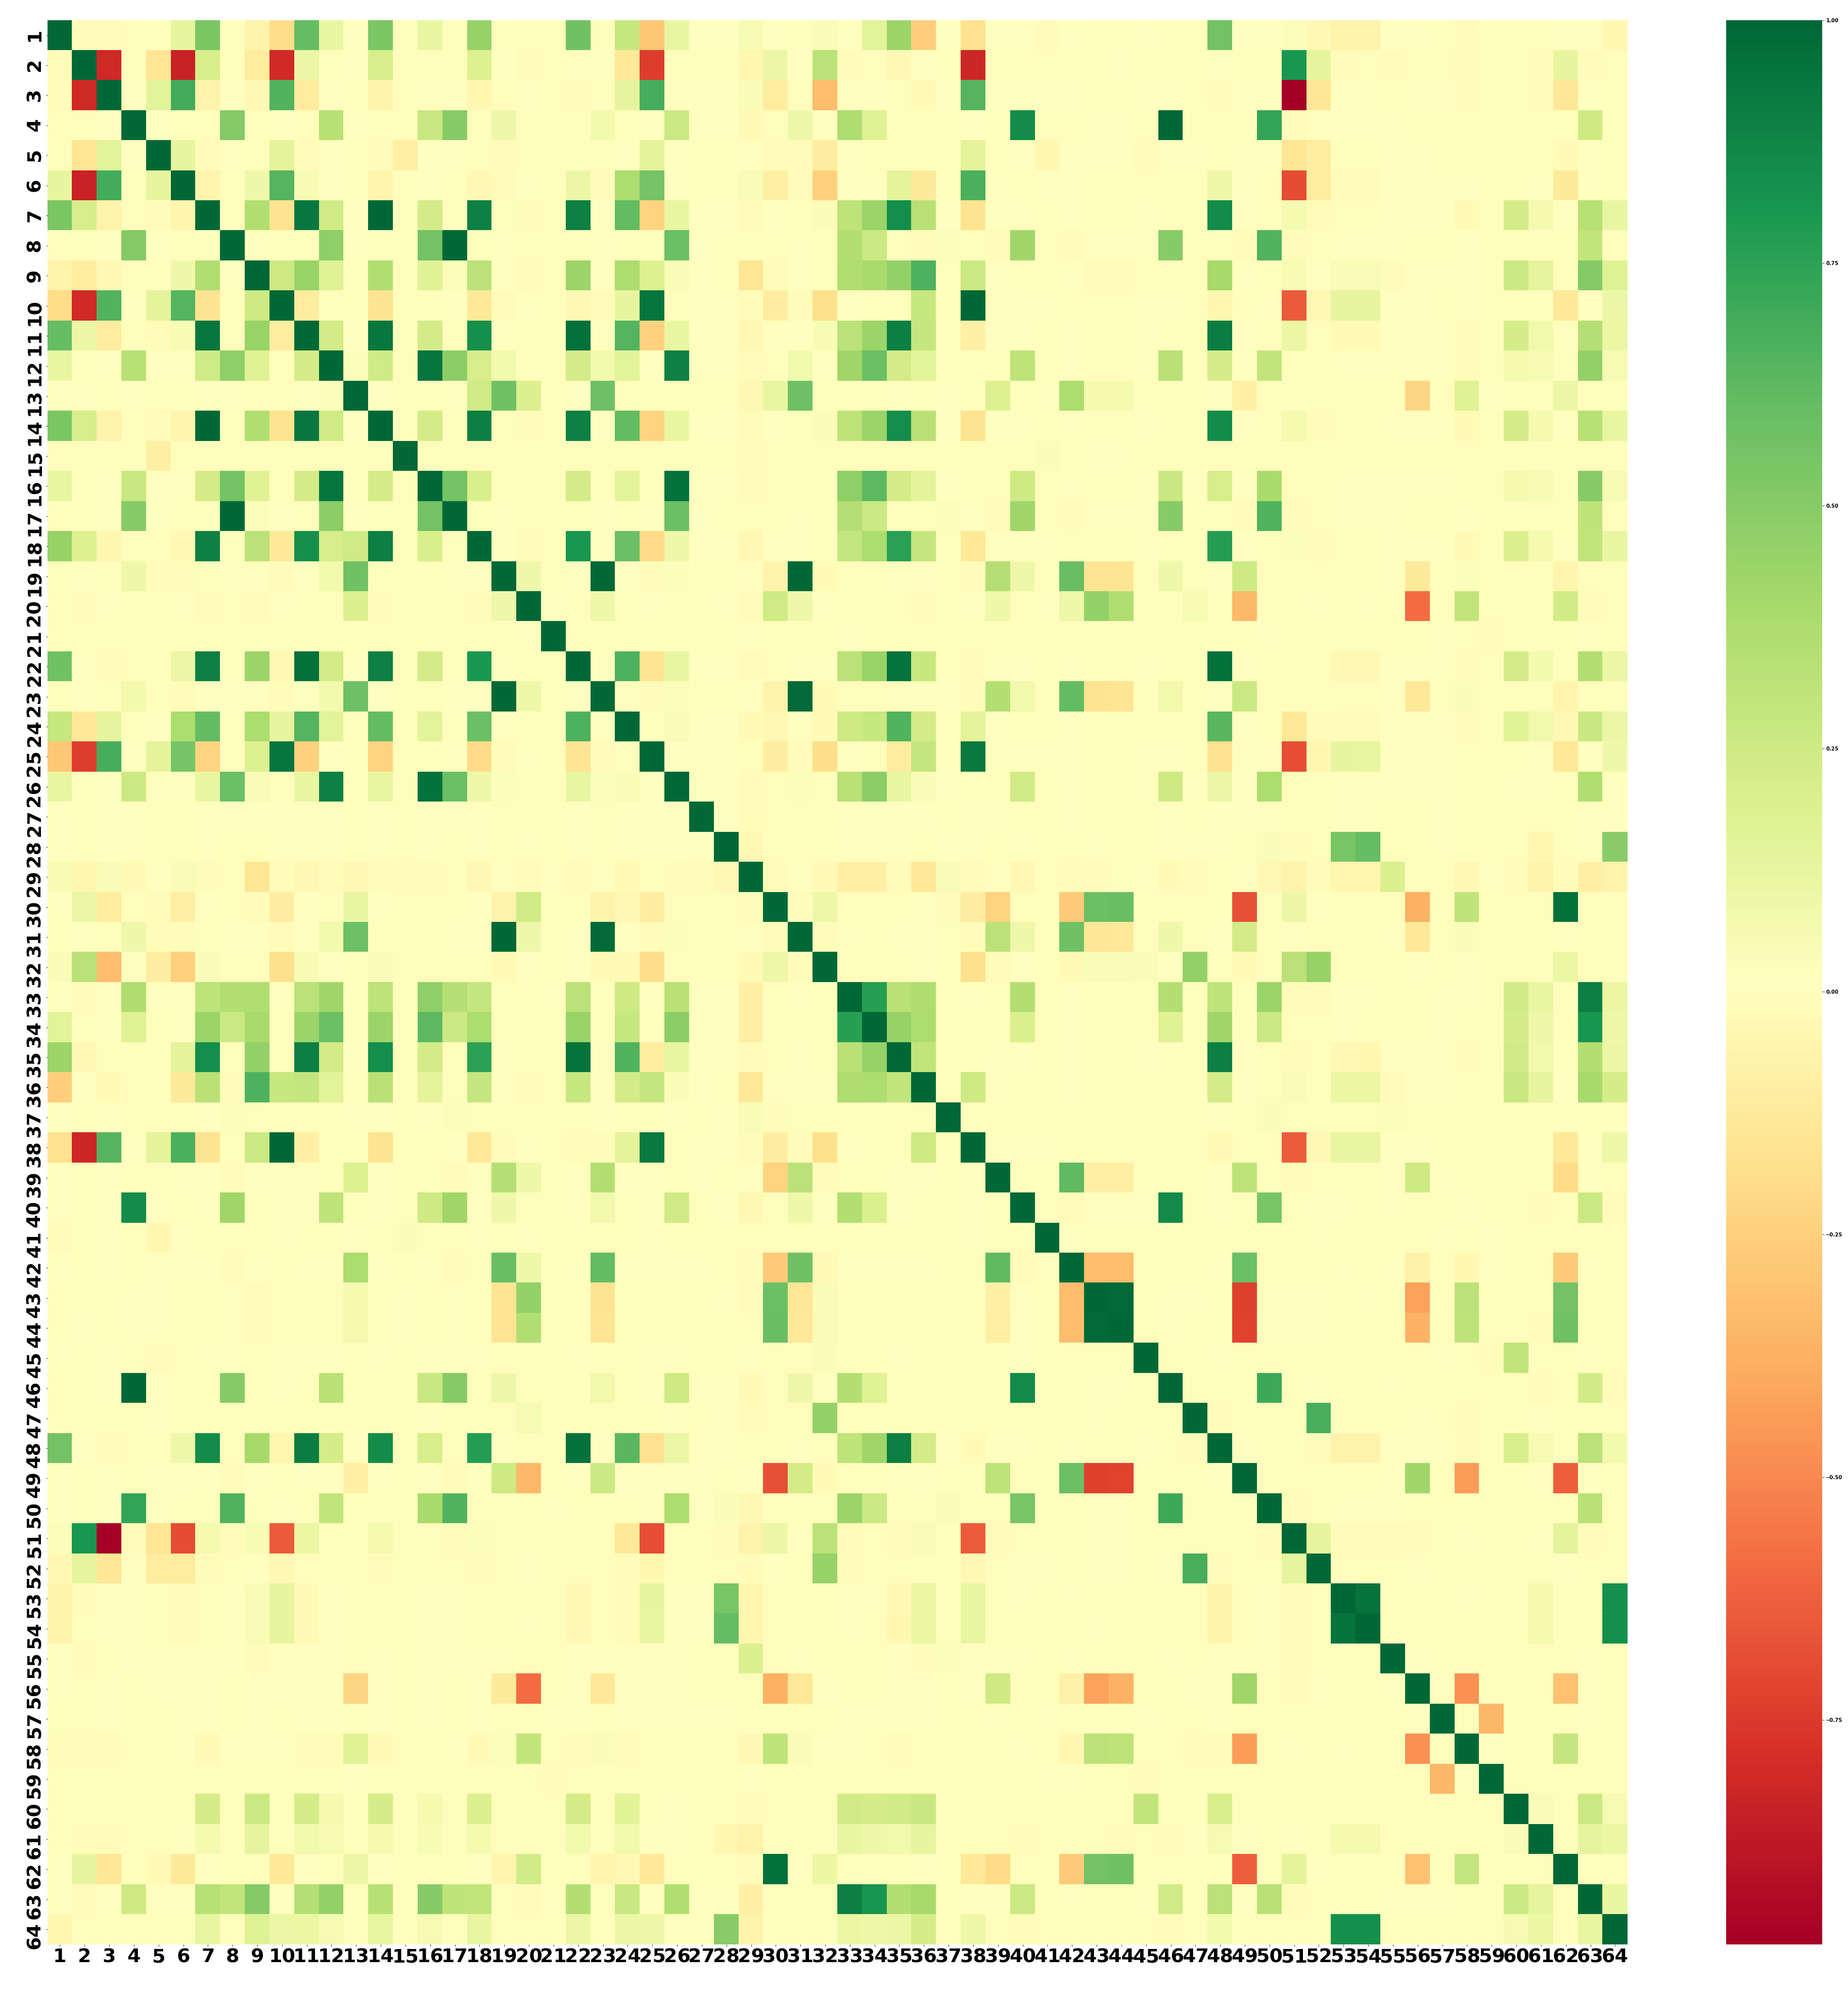
\includegraphics[width=2\columnwidth]{correlation_crop.png}
\caption{\label{fig::correlation} Correlation matrix for the dataset}
\end{figure*}

% \section{List of parameters for fine-tuning models}
% \label{app::params}


\end{document}
